\documentclass{article} % For LaTeX2e
\usepackage{iclr2027_conference,times}

\usepackage[hyphens]{url}
\usepackage{graphicx}
\usepackage{multirow}
\usepackage{amsmath}
\usepackage{amssymb}
\usepackage[table]{xcolor}
\usepackage{caption}
\usepackage{booktabs}
\usepackage{pifont} % circled-number badges for the teaser/method legends
\setlength{\marginparwidth}{2cm}
\usepackage{todonotes}
\usepackage{float}

% --- Badge colors for the teaser figure legend (colors match figs/tiser.pdf) ---
\definecolor{tsrGreen}{HTML}{41CE54}
\definecolor{tsrCyan}{HTML}{41CBCE}
\definecolor{tsrOlive}{HTML}{C9CE41}
\definecolor{tsrMagenta}{HTML}{DE6DD7}
\definecolor{tsrYellow}{HTML}{F7F13F}
\newcommand{\badgeimg}{\textcolor{tsrGreen}{\ding{182}}}   % (1) images + poses
\newcommand{\badgemesh}{\textcolor{tsrCyan}{\ding{183}}}   % (2) meshes
\newcommand{\badgegmm}{\textcolor{tsrOlive}{\ding{184}}}   % (3) 2D Gaussian mixture
\newcommand{\badgeenv}{\textcolor{tsrMagenta}{\ding{185}}} % (4) hierarchical env map
\newcommand{\badgekan}{\textcolor{tsrYellow}{\ding{186}}}  % (5) KAN
% --- Badge colors for the method pipeline figure (fig:method); colors match figs/method.pdf ---
\definecolor{mtdCoral}{HTML}{E26A64}
\definecolor{mtdBlue}{HTML}{6ABCE2}
\definecolor{mtdGreen}{HTML}{4FD370}
\definecolor{mtdPurple}{HTML}{AE6AE2}
\definecolor{mtdOrange}{HTML}{E57A08}
\newcommand{\mtdone}{\textcolor{mtdCoral}{\ding{182}}}    % 1 manifold position
\newcommand{\mtdtwo}{\textcolor{mtdBlue}{\ding{183}}}     % 2 Euclidean position
\newcommand{\mtdthree}{\textcolor{mtdBlue}{\ding{184}}}   % 3 normal
\newcommand{\mtdfour}{\textcolor{mtdBlue}{\ding{185}}}    % 4 view
\newcommand{\mtdfive}{\textcolor{mtdGreen}{\ding{186}}}   % 5 adaptive env map
\newcommand{\mtdsix}{\textcolor{mtdPurple}{\ding{187}}}   % 6 diffuse color
\newcommand{\mtdseven}{\textcolor{mtdPurple}{\ding{188}}} % 7 reflectivity weight
\newcommand{\mtdeight}{\textcolor{mtdOrange}{\ding{189}}} % 8 specular color

\title{Automatic Neural Baking}

% Authors must not appear in the submitted version. They are hidden
% as long as the \iclrfinalcopy macro remains commented out below.
\author{Anonymous Authors}

%\iclrfinalcopy % Uncomment for camera-ready version, but NOT for submission.
\begin{document}


\maketitle


\begin{abstract}
Baking precomputes an object's appearance into a texture on a mesh, but baked formats cannot
represent sharp view-dependent reflection. Neural and splat representations can, yet they place
appearance in the space \emph{around} the object rather than on its surface, so there is nothing to
bake. We identify two independent obstructions to the natural fix, binding splats to the faces of a
known mesh, and prove both are fundamental rather than incidental. First, coplanar primitives admit
no compositing order that is both view-stable and geometrically meaningful, and no cheap,
per-primitive perturbation of the depth, such as a normal offset, can repair this. Second,
reflection about a fixed normal is a rotation of the view sphere, so any per-primitive
view-dependent color model is band-limited at a fragment regardless of how many primitives are
used: adding primitives adds no angular bandwidth. We resolve both with Automatic Neural Baking, a construction that works rather than the only one
that could. An \emph{on-manifold kernel field}, 2D Gaussian disks anchored to mesh faces and
blended by an order-free partition of unity, removes the ordering obstruction; factoring view
dependence out of the elements into a shared environment map and a FastKAN decoder removes the
locality bound. The result composes directly with the traditional rendering pipeline, baking
splat-quality, real-time appearance onto a mesh.
\end{abstract}

\section{Introduction}
% --- Teaser figure ---------------------------------------------------
% Placed directly below the author block and above the abstract, as in
% the original submission. Edit the caption/label below.
\begin{figure}[t]
\centering
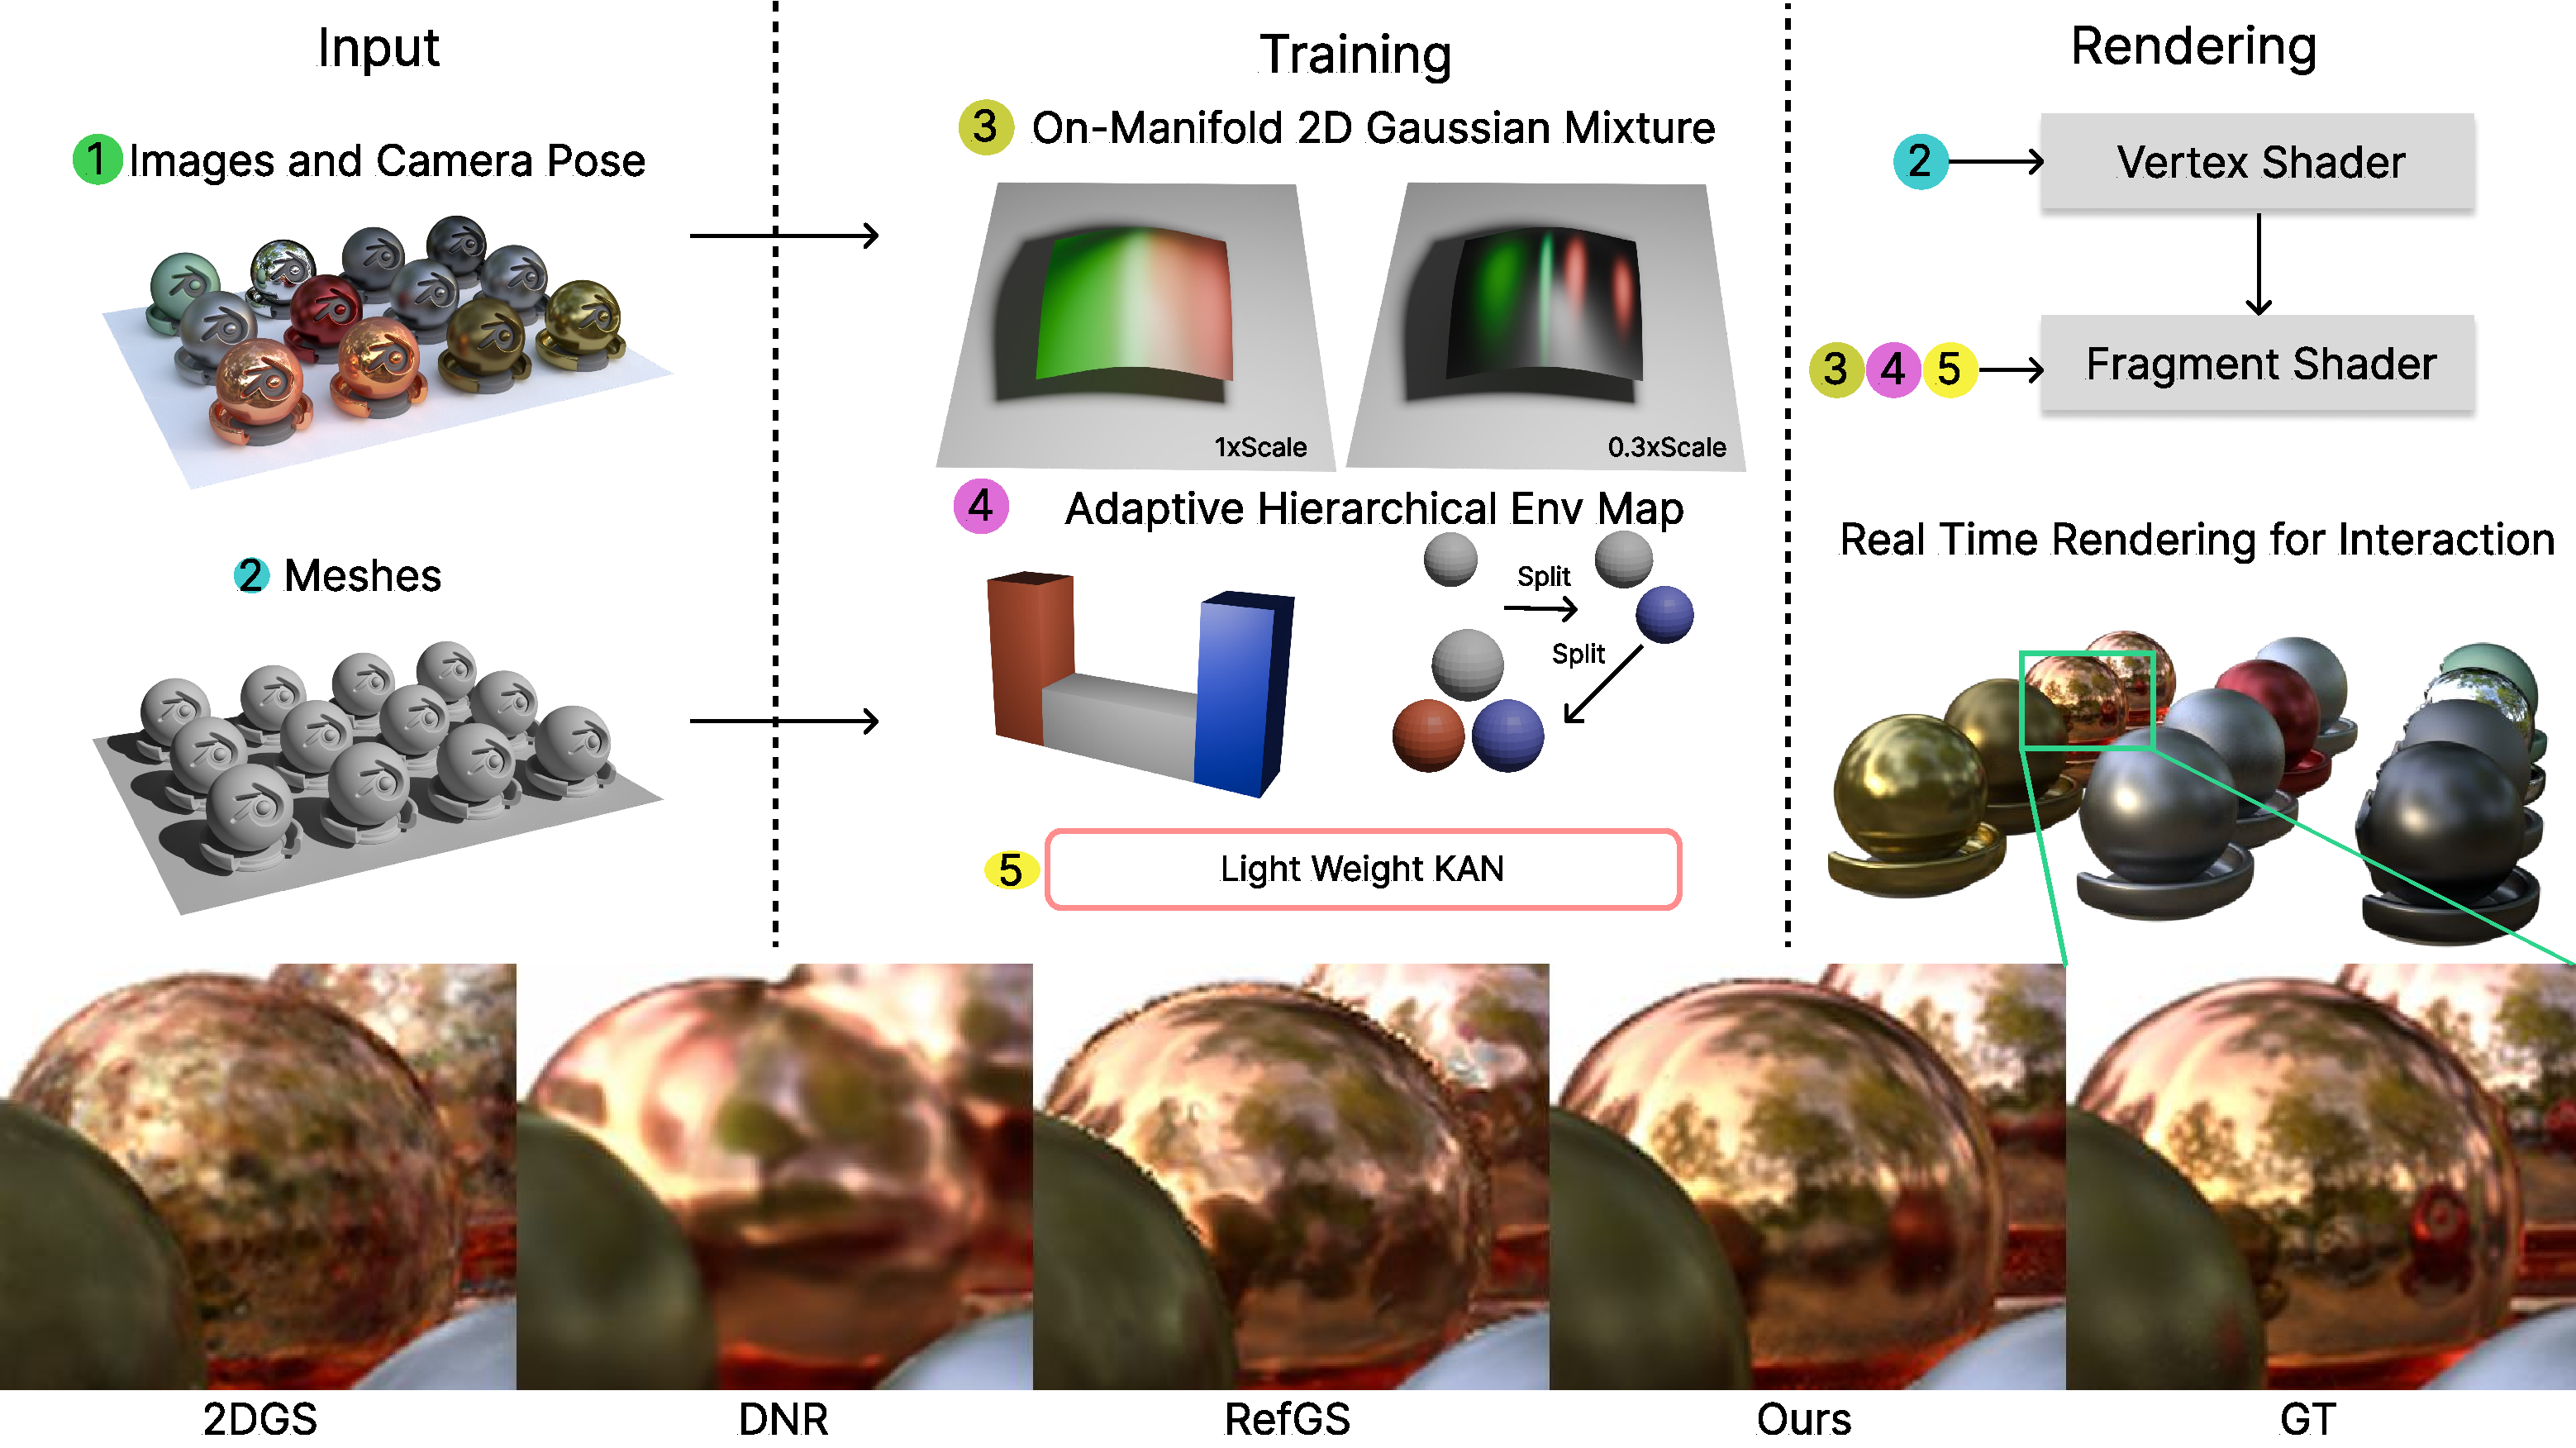
\includegraphics[width=\linewidth]{figs/tiser.pdf}
\caption{%
\textbf{Automatic Neural Baking bakes highly reflective, view-dependent appearance directly onto a mesh, rendering it in real time (>60 FPS) with fidelity that surpasses state-of-the-art flexible-mesh methods.}
\emph{Comparison}: on Shiny-Blender, our method reproduces sharp, high-frequency specular reflections that 2DGS~\citep{2DGS} and DNR~\citep{DNR} smears and that RefGS~\citep{refgs} recovers less crisply, while running natively in a standard rasterizer rather than requiring depth-sorted splat rendering.
\emph{Pipeline}: from posed reference images ~\badgeimg{} and the corresponding triangle mesh~\badgemesh, we optimize three interchangeable, rasterizer-native modules - an on-manifold 2D Gaussian mixture storing diffuse albedo and reflectivity~\badgegmm, an adaptive, hierarchical environment map capturing self-reflection ~\badgeenv; and a lightweight KAN that evaluating the reflection equation for far-field specular~\badgekan - all evaluated per-fragment in a standard fragment shader
\badgemesh\,\badgegmm\,\badgeenv\,\badgekan.%
}
\label{fig:teaser}
\end{figure}
% ----------------------------------------------------------------------

Interactive applications such as games, virtual reality, and other online rendering, demand photorealistic imagery in real time (typically $\geq 60$~FPS).
The standard baking-and-rasterization pipeline meets this by precomputing appearance offline into textures over the mesh, which a fragment shader then samples cheaply at run time~\citep{RealTimeRendering}.


Automating this stage, however, remains hard for the shiny, view-dependent materials that matter most:
the usual baked formats, for instance, lightmaps or low-order Spherical Harmonic (SH) probes, store only smooth, view-independent lighting and miss angle-dependent highlights~\citep{AllFrequency, curveSurfaces, nerfTexture}.
Baking also presupposes a global UV atlas, whose automatic construction remains fragmented and largely manual~\citep{Levy2002LSCM, poranne2017autocuts, li2018optcuts, srinivasan2024nuvo}. Per-face texturing such as Ptex~\citep{ptex} removes the UV atlas, but as a static texture it still cannot capture high-frequency, view-dependent reflection.
The seminal automatic neural baking method is Deferred Neural Rendering (DNR)~\citep{DNR}, which bakes learned neural textures onto a mesh and decodes them at render time.
However, DNR shares the same weakness as classical baking and cannot reproduce high frequency view-dependent color.
Our method is a direct, modern successor to it: The mesh is an input, not an output; in our setting it is an artist-authored asset, the standard target of baking workflows. Like DNR, it is a traditional baking method that produces a baked mesh asset. Unlike DNR, it also captures the sharp, view-dependent appearance that baking has always lacked. 

Such appearance has instead been the domain of neural and splat representations. Neural Radiance
Fields (NeRFs)~\citep{NeRFVanilla} and 3D Gaussian Splatting (3DGS)~\citep{3DGS} have
revolutionized novel view synthesis, reaching a photorealism that classical baking cannot match by
treating the scene as a continuous optimization problem.
But they place appearance in the \emph{ambient space}: a continuous field over $\mathbb{R}^3$ for
NeRF, a mixture of anisotropic kernels for 3DGS.
The baking pipeline instead treats an object as a \emph{surface}, a two-dimensional manifold
$\mathcal{M}\subset\mathbb{R}^3$ carrying appearance as a field on $\mathcal{M}$ itself.
Because the ambient field for NeRF and 3DGS has no 2D domain, there is nothing to bake.

Attempts to close this gap do not change the domain. Extraction methods recover a mesh after the
fact~\citep{sugar, gaussianSurfels} but only approximate a surface the representation never carried,
and the primitives themselves remain free in $\mathbb{R}^3$.
2DGS~\citep{2DGS} flattens each ellipsoid into a disk, collapsing the kernel across its normal
direction; this removes thickness, but a sum of such disks scattered through space is still an
ambient-space distribution.
The natural remaining step is to bind the primitives directly to the faces of a known mesh. This is
where the difficulty becomes concrete.

Once primitives are strictly coplanar, their depth keys tie and alpha compositing has no
well-defined order. The standard remedies fail in instructive ways.
Offsetting disk $i$ along the face normal by $\varepsilon_i$ separates two disks by
$(\varepsilon_i-\varepsilon_j)(\mathbf{n}\cdot\mathbf{v})$, where n is the normal of that face, and v is the viewing direction. 
The order changes at grazing angles: small
offsets reproduce the tie, while large ones yield an ordering that flips as the camera orbits, so
gradients from different views disagree about which primitive owns a fragment.
Large offsets also let the optimizer reintroduce extent along $\mathbf{n}$, reinstating the ambient
drift the binding was meant to remove and degrading the surface it is bound to.
Breaking ties by a fixed primitive index is view-stable but imposes an occlusion relation
uncorrelated with geometry.
The obstruction is not depth but \emph{order-dependence itself}: on a single opaque surface no
ordering is both view-stable and geometrically meaningful.


We therefore drop ordering altogether. We bake appearance as an \emph{element-wise field whose
domain is the surface}: a mixture of two-dimensional Gaussian disks anchored to mesh faces in
barycentric coordinates, blended at each fragment by a normalized partition of unity over the $K$
nearest disks. Because the blend is a convex combination rather than an alpha composite, it is
invariant to order; the global $O(N\log N)$ sort becomes an $O(K)$ local gather, with no degeneracy
to avoid. This is a texture in a sense that a neural raster atlas~\citep{DNR} is not: its elements
are individually addressable, movable, mergeable, and differentiable, and it needs no UV atlas. To
our knowledge it is the first differentiable element-wise appearance field defined on the manifold
itself.

On this field we place two modules supplying the view-dependent term: an adaptive hierarchical
environment map that splits the object into near-convex parts, so self-reflection reduces to a local
lookup rather than a secondary ray; and a compact FastKAN decoder~\citep{fastkan, kan} that
interpolates the reflection from sparse views. All three modules are interchangeable, and each is
evaluated per fragment against a single opaque surface. The representation is read and written like
a texture: we demonstrate it in nvdiffrast at over 60 FPS.



The appearance at each surface point is thus a local diffuse color plus a single gated reflection
covering both far-field and near-field (self-)reflection, composited in logit space.
On Shiny-Blender this reaches $36.99$\,dB PSNR; starting instead from an imperfect reconstructed
mesh, optimizing appearance alone also improves that mesh's normal error and Chamfer distance on
every scene.

Our central contribution is the representation; the remaining items are properties it makes
possible.
\begin{itemize}
\item \textbf{An element-wise texture on a 2-manifold.} A differentiable appearance field whose
domain is the mesh surface and whose blending is order-independent, requiring no UV atlas and no
depth sort: an $O(K)$ per-fragment gather replaces the global $O(N\log N)$ sort. We diagnose why
face-bound splats cannot achieve this and measure each failure mode (Sec.~\ref{sec:ablation}).
The surface kernel is interchangeable; we adopt a 2D Gaussian mixture as a strong default
(Sec.~\ref{sec:gmm}).
\item \textbf{Sharp view-dependent appearance, baked.} A FastKAN decoder over an adaptive
hierarchical environment map captures high-frequency specularity, and near-convex decomposition
reduces self-reflection to a local lookup rather than a secondary ray. On Shiny-Blender we reach
$36.99$\,dB PSNR, the best reported result given the same geometry.
\item \textbf{Refining the mesh through appearance alone.} The anchoring that makes the field a
surface parameterization also makes its gradient blind along the surface normal: a disk can ask the
mesh to slide, never to move in or out. We recover that direction by momentarily reading each disk's
gradient in the ambient space the anchoring excludes, then pulling it back onto the vertices through
the same barycentric weights that reconstructed the disk. In this way, the mesh moves while the appearance
field stays a parameterization of it. Starting from a reconstructed mesh~\citep{refgs}, this
improves normal MAE$^\circ$, Chamfer distance, and F1 on all six Shiny-Blender scenes.
\item \textbf{Evaluable in a fragment shader.} Every module is a local, per-fragment operation over
a single opaque surface  without global state, and secondary rays. The representation is therefore
shader-implementable by construction; we realize it in nvdiffrast and render both datasets at over
$60$ FPS.
\end{itemize}
\section{Related Work}

\subsection{Baking Appearance onto Explicit Geometry}
Baking precomputes an object's appearance into reusable textures~\citep{RealTimeRendering}.
Deferred Neural Rendering generalized this recipe by storing learned feature textures on the mesh and decoding them in screen space~\citep{DNR}.
With the advent of NeRF~\citep{NeRFVanilla}, baking became a conversion problem:
trained fields are distilled into sparse feature grids~\citep{bakingNeRF}, textured polygon soups~\citep{MobileNeRF}, watertight meshes~\citep{bakedSDF}, or deformable avatars~\citep{bakedAvatar},
as well as differentiable inverse rendering recovers meshes, materials, and lighting directly from images~\citep{nvdiffrec},
and neural textures can be synthesized over curved surfaces~\citep{nerfTexture}.
These methods deliver genuine assets, but their view-dependent capacity is an afterthought:
low-order SH lobes or small per-pixel decoders biased toward diffuse content.
Our pipeline retains the deferred, texture-like structure of this line
while devoting explicit model capacity to sharp specularity.
In addition, methods above presuppose a global UV atlas,
whose seam-cutting and packing remain tedious to author and non-differentiable to optimize;
by anchoring appearance in per-face barycentric coordinates, our formulation sidesteps this requirement entirely. Per-face texturing such as Ptex~\citep{ptex} likewise removes the atlas, but its static per-face textures cannot represent the high-frequency, view-dependent reflection that continuous splat representations later captured.

\subsection{Modeling View-Dependent Appearance}
A parallel line of work asks how to reconstruct sharp specular transport in the first place.
Ref-NeRF reparameterizes outgoing radiance about the reflected view direction,
substantially improving specular fidelity within a volumetric field~\citep{refnerf}.
In the splatting regime, recent methods evaluate reflections in screen space against a learned environment map:
GaussianShader attaches simplified shading functions to each splat~\citep{gaussianShader},
3DGS-DR defers reflection evaluation to a per-pixel normal buffer~\citep{3dgsDR},
Ref-Gaussian incorporates physically based deferred shading~\citep{refgs},
and Spec-Gaussian replaces spherical harmonics with anisotropic spherical Gaussians~\citep{specGaussian}.

Whether it is an evaluated BRDF~\citep{cookTorrance} against a prefiltered environment map, as in classical real-time physically based shading~\citep{karis2013pbr, RealTimeRendering},
or learned as above, environment-map reflection shares one limitation: it assumes all incident light arrives from infinitely far away.
Reducing a reflection to a single directional lookup, it cannot represent near-field self-reflection or self-occlusion, the light an object casts back onto itself.
Recovering these effects generally requires tracing secondary rays~\citep{refgs, 3dgsRayTracing}, which reintroduces the very queries that rasterization avoids.
We instead handle self-reflection geometrically: because a convex part can neither occlude nor reflect itself,
we split an object into near-convex parts via convex decomposition~\citep{coacd}, each carrying its own environment map,
grown as an adaptive hierarchy that isolates high-error regions, so that self-reflection reduces to local lookups rather than recursive rays.

These methods solve specular \emph{reconstruction}, yet all of them operate on free-form primitives in ambient $\mathbb{R}^3$:
they expose no solid surface, retain the global depth sort,
and produce nothing that can be baked onto a given mesh.
Naively binding them to a fixed surface only forces them co-planar and destabilizes the sort;
our surface-bound 2D formulation sidesteps this by construction, requiring no sorting at all.
\begin{figure}[t]
    \centering
    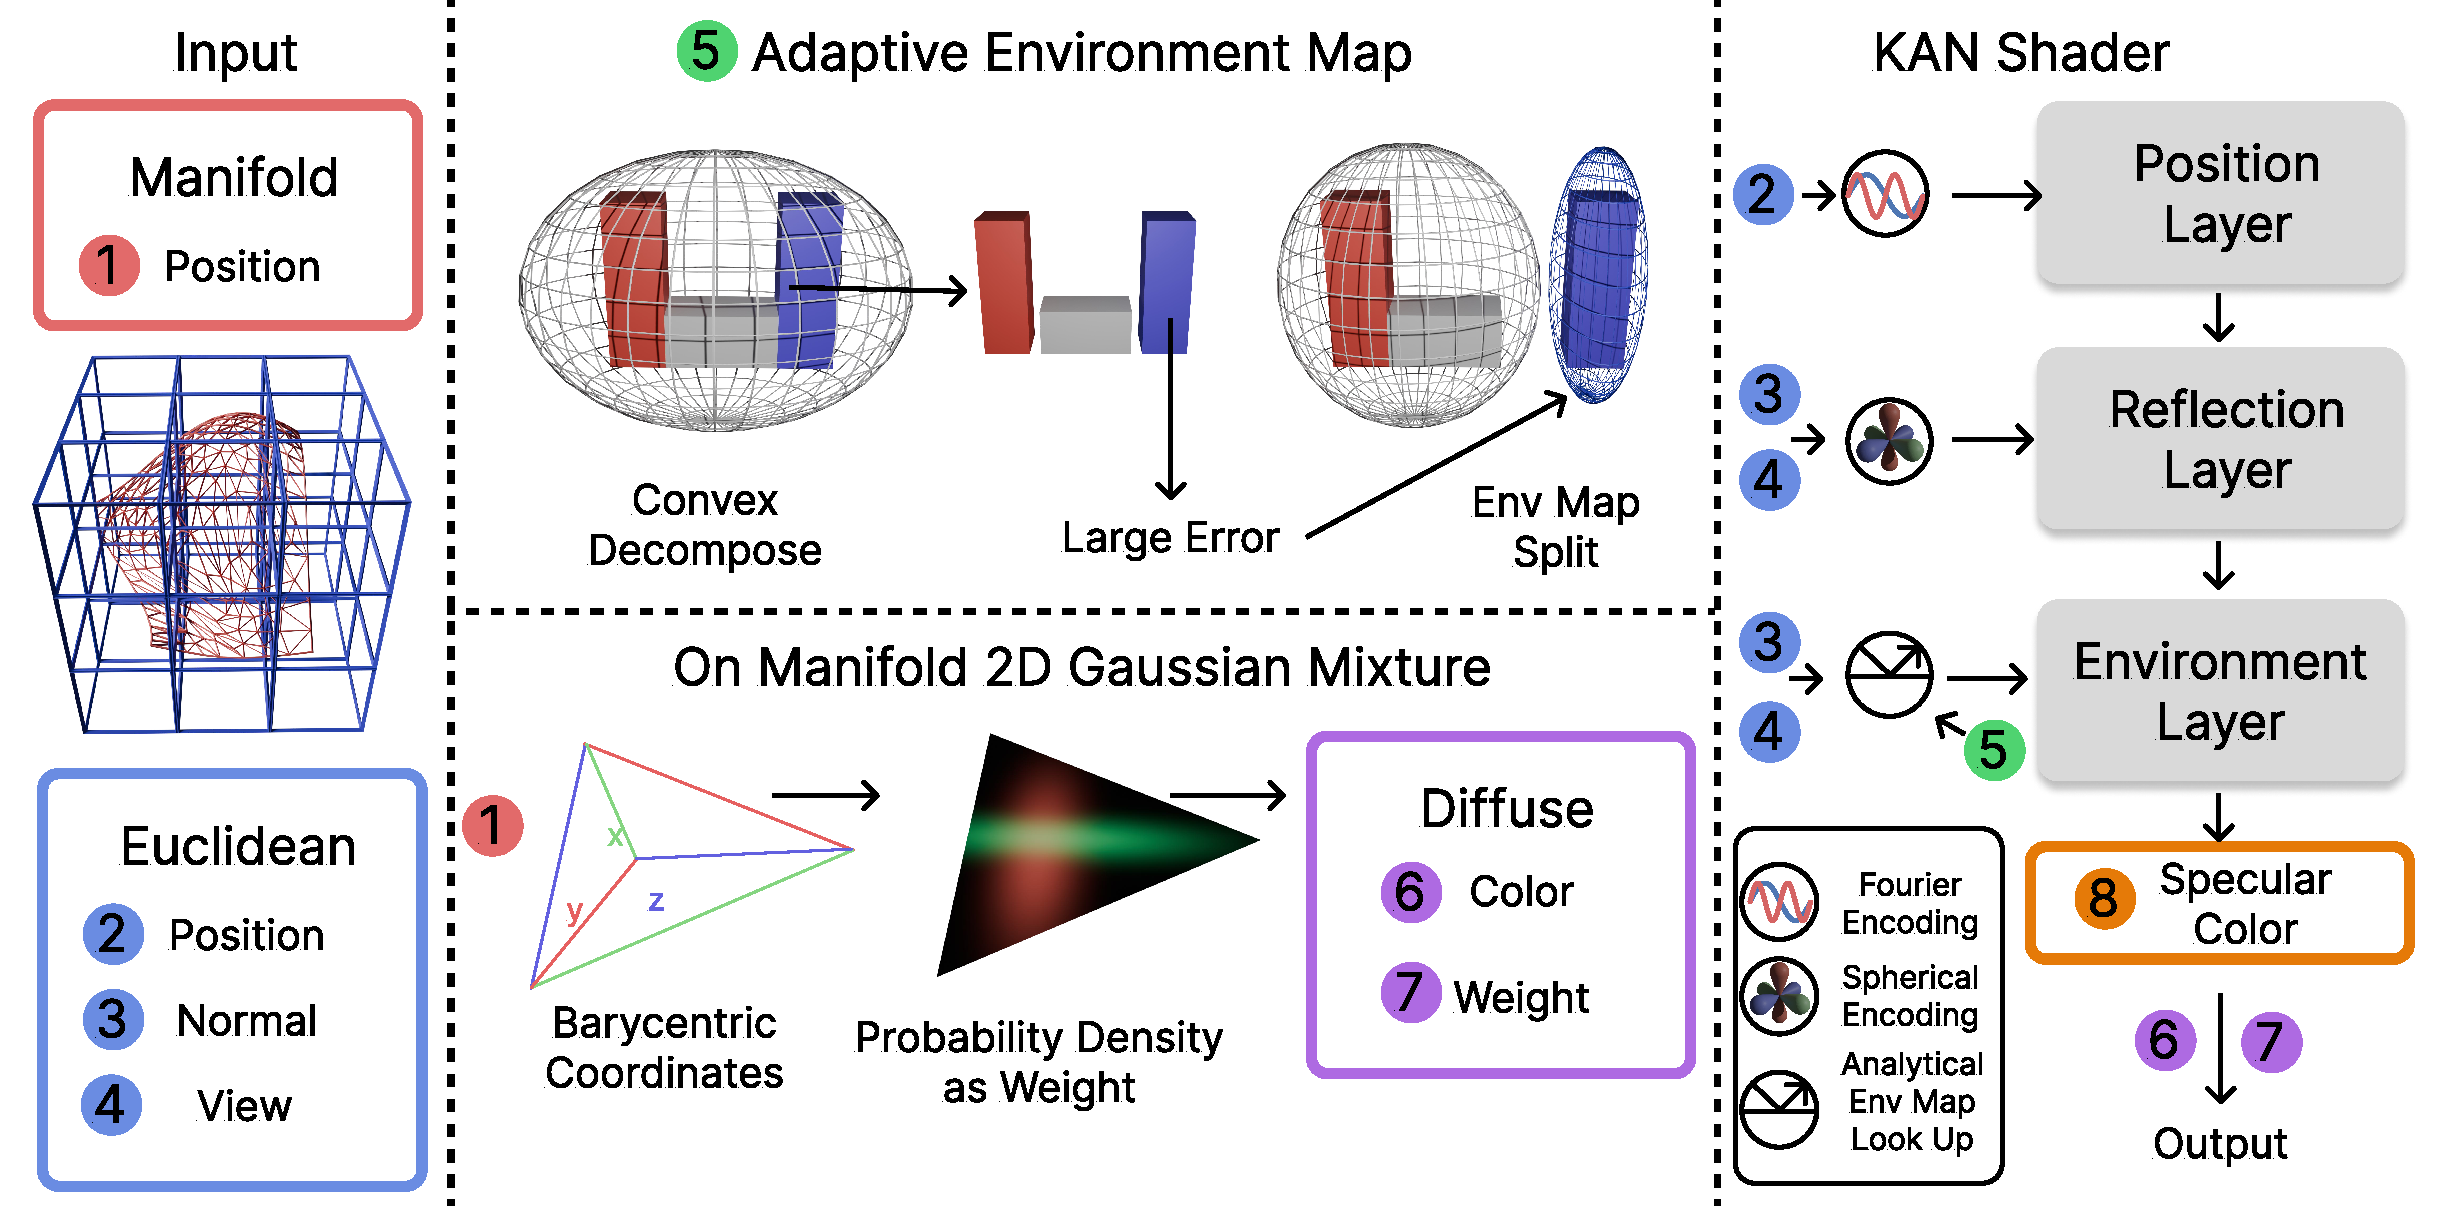
\includegraphics[width=\linewidth]{figs/method.pdf}
    \caption{%
    \textbf{Pipeline overview.}
    \emph{Input:} two position types---the on-manifold surface position \mtdone{} (barycentric coordinates on a mesh face) and the Euclidean position \mtdtwo{}, plus the surface normal \mtdthree{} and view direction \mtdfour{}.
    \emph{On-manifold 2D Gaussian mixture} (Sec.~\ref{sec:gmm}): from the barycentric position \mtdone{} we gather nearby surface Gaussians by their probability density (a partition-of-unity weight), giving the diffuse color \mtdsix{} and per-point reflectivity \mtdseven{}.
    \emph{Adaptive environment map} \mtdfive{} (Sec.~\ref{sec:env}): the object is convex-decomposed into near-convex parts, and the highest-error region is recursively split off into its own map.
    \emph{KAN shader} (Sec.~\ref{sec:kan}): a FastKAN decoder consumes the Fourier-encoded position \mtdtwo{} (Position Layer), the spherically-encoded normal \mtdthree{} and view \mtdfour{} (Reflection Layer), and an analytical lookup into the environment map \mtdfive{} (Environment Layer), producing the specular color \mtdeight{}.
    \emph{Output:} the final color composites the specular \mtdeight{} with the diffuse color \mtdsix{} gated by the reflectivity \mtdseven{}, i.e.\ Eq.~\eqref{eq:appearance}.%
    }
    \label{fig:method}
    \vspace{-4mm}
\end{figure}

\subsection{Attaching Radiance Fields to Surfaces}
A third line pushes radiance distributions toward surfaces.
Flattened kernels such as 2D Gaussian disks~\citep{2DGS} and Gaussian surfels~\citep{gaussianSurfels}
collapse one axis of the kernel to improve geometric accuracy, yet the primitives still float freely in $\mathbb{R}^3$. Mesh-scaffolded methods go further: SuGaR regularizes splats toward an extracted mesh~\citep{sugar},
GaMeS parameterizes Gaussians on triangle faces to enable editing~\citep{games},
SplattingAvatar embeds splats in a deformable template for animation~\citep{splattingAvatar},
and Texture-GS learns a UV mapping so that a 2D texture colors the splats~\citep{textureGS}.
In every case, however, the mesh merely \emph{drives} the kernels:
the rendered primitives remain three-dimensional, ambient-space objects composited by depth sorting,
and the domain of the appearance field never becomes the surface itself.
\citet{neumesh} bind learnable codes on the vertices, but never allow the code representation to float inside the 2D manifold.
The original EWA surface splatting~\citep{EWA} is, moreover, not differentiable.
In contrast, we define a strictly 2D, sort-free Gaussian mixture expressed in the barycentric coordinates on  the faces that is differentiable and free inside the 2D manifold.
In this way the mesh is not scaffolding but the domain, and it remains the authoritative solid geometry for collision, physics, and animation.



\section{Method}
\subsection{Overview}

Given a triangle mesh and a set of posed reference images, we bake the object's appearance into a field that a rasterizer can evaluate per fragment in real time. The mesh is fixed; only the appearance on it is optimized. Sec.~\ref{sec:downstream} then describes two downstream tasks the baked asset supports, neither of
which alters the pipeline above.

We bake appearance with three interchangeable modules and composite their outputs at each fragment.
An on-manifold 2D Gaussian mixture (Sec.~\ref{sec:gmm}) carries the view-independent fields; an
adaptive environment map (Sec.~\ref{sec:env}) supplies the incident radiance, including the light
the object casts on itself; and a compact FastKAN decoder (Sec.~\ref{sec:kan}) turns a lookup into
that map into a view-dependent reflection. At a visible surface point $\mathbf{x}$ seen along view
direction $\mathbf{v}$, the three combine as
%
\begin{equation}
c(\mathbf{x}, \mathbf{v}) = \operatorname{sigmoid}\!\Big( \operatorname{logit}\big(a(\mathbf{x})\big)
+ m(\mathbf{x})\, r(\mathbf{x}, \mathbf{v}) \Big),
\label{eq:appearance}
\end{equation}
%
where the albedo $a(\mathbf{x})\in[0,1]^3$ and the reflectivity $m(\mathbf{x})\in[0,1]$ are read
from the mixture ($m{=}0$ matte, $m{=}1$ mirror) and the residual $r(\mathbf{x},\mathbf{v})$ is
emitted by the decoder. Compositing in logit space lets the reflection act as an additive residual
on the diffuse base while keeping the result in $[0,1]$ without clamping; $m$ gates where it
applies. 

\subsection{2D Gaussian Mixture on the Manifold}
\label{sec:gmm}
The albedo and reflectivity fields are stored by a mixture of $N$ two-dimensional Gaussian
``disks'' on the mesh surface ($N{=}10^6$ in our experiments). $N$ is fixed at initialization and
never changes during training: there is no densification, pruning, or opacity culling. The count can
be reduced after training, without retraining, by the compaction of Sec.~\ref{sec:Compaction}.

\paragraph{On-manifold anchoring.}
Each disk $i$ is assigned to a single triangle $f_i$ and a barycentric coordinate
$\mathbf{b}_i=(b_{i,0},b_{i,1},b_{i,2})$ with $b_{i,k}\ge 0$ and $\sum_k b_{i,k}=1$.
Its center is \emph{reconstructed} from the live vertices of that triangle,
%
\begin{equation}
\mathbf{x}_i = b_{i,0}\,\mathbf{p}_0(f_i) + b_{i,1}\,\mathbf{p}_1(f_i) + b_{i,2}\,\mathbf{p}_2(f_i),
\label{eq:center}
\end{equation}
%
so $\mathbf{x}_i$ is by construction a convex combination of the face's vertices and lies exactly on
the triangle. The face therefore supplies the disk's frame as well as its position: its extent lives
in the in-plane axes $(\mathbf{t}_1,\mathbf{t}_2)$ of $f_i$, with an in-plane rotation $\theta_i$
about the face normal $\mathbf{n}$ and an anisotropic in-plane scale $(s_{i,1},s_{i,2})$. We give
the disk \emph{no extent along} $\mathbf{n}$, so it is a strictly two-dimensional element rather
than a three-dimensional one with a constrained center.

\paragraph{Per-disk attributes.}
Each disk carries two view-independent attributes: an albedo $a_i\in[0,1]^3$ and a scalar reflectivity $m_i\in[0,1]$, both stored as unconstrained logits and squashed at use.
The continuous fields $a(\mathbf{x})$ and $m(\mathbf{x})$ in Eq.~\eqref{eq:appearance} are obtained by blending these per-disk attributes over the disks near $\mathbf{x}$ (described next).

\paragraph{Partition-of-unity blend.}
A fragment at $\mathbf{x}$ on face $f$ gathers from $\mathcal{N}(f)$, the fixed set of the $K{=}16$ disks nearest that face. These disks are not restricted to $f$: the top-$K$ set spans $f$ and its neighboring faces, so the gather crosses face boundaries rather than being truncated per face. Each disk is weighted by its own Gaussian density at $\mathbf{x}$, evaluated in the disk's tangent frame:
\begin{equation}
w_k(\mathbf{x}) = \exp\!\Big(-\tfrac12\big[(u_{k,1}/s_{k,1})^2 + (u_{k,2}/s_{k,2})^2\big]\Big), \quad
\bar{w}_k(\mathbf{x}) = w_k(\mathbf{x}) \Big/ \sum_{j\in\mathcal{N}(f)} w_j(\mathbf{x}),
\label{eq:pou}
\end{equation}
where $u_{k,j}=(\mathbf{x}-\mathbf{x}_k)\cdot\mathbf{t}_{k,j}$ is the fragment's in-plane offset from disk $k$'s center along its tangent axis $\mathbf{t}_{k,j}$. The per-fragment fields are the resulting convex combination,
\begin{equation}
a(\mathbf{x}) = \sum_{k\in\mathcal{N}(f)} \bar{w}_k(\mathbf{x})\, a_k,  \quad
m(\mathbf{x}) = \operatorname{sigmoid}\!\Big(\sum_{k\in\mathcal{N}(f)} \bar{w}_k(\mathbf{x})\, \operatorname{logit}(m_k)\Big),
\label{eq:blend}
\end{equation}
with $a_k,m_k$ the squashed per-disk albedo and reflectivity. The weights form a partition of unity
($\sum_k \bar{w}_k = 1$), so each field is a \emph{normalized} convex combination of the nearby
disks rather than an alpha composite. This is the order-independence the representation was designed
around (Sec.~\ref{sec:intro}): the blend never asks which disk lies in front, so the coplanar depth
ties cannot arise and the $\mathcal{O}(K)$ gather needs no sort.

\subsection{Adaptive Environment Map}
\label{sec:env}
We describe the reflection lookup first without its learned parts, where it is ordinary environment mapping: a directional fetch and a weighted blend.

\paragraph{Fetching}
Treat the environment as a classical equirectangular map. At a surface point with normal $\mathbf{n}$ seen from view direction $\mathbf{v}$, the mirror-reflected direction is $\boldsymbol{\omega}_r = 2(\mathbf{n}\cdot\mathbf{v})\,\mathbf{n} - \mathbf{v}$. We then start a longitude--elevation coordinate and bilinearly sample according to the direction.

\paragraph{Which map: near-convex parts.}
A single global map assumes all light arrives from infinitely far away, so it cannot reproduce the
light an object casts on itself. We resolve this geometrically. Within a convex part there is no
self-occlusion and no self-reflection, so all incident light is external and a single directional
map is a good approximation; what a global map cannot capture is the light exchanged \emph{between}
parts. We therefore split the object into near-convex parts with a convex
decomposition~\citep{coacd} and give each part its own map, so that light reaching a part from the
rest of the object is absorbed into that part's map and read back as an ordinary far-field lookup.
The approximation is that this inter-part light is treated as distant and position-independent
within a part, and
Sec.~\ref{sec:ablation} measures what it recovers.
\begin{figure}[t]
    \centering
    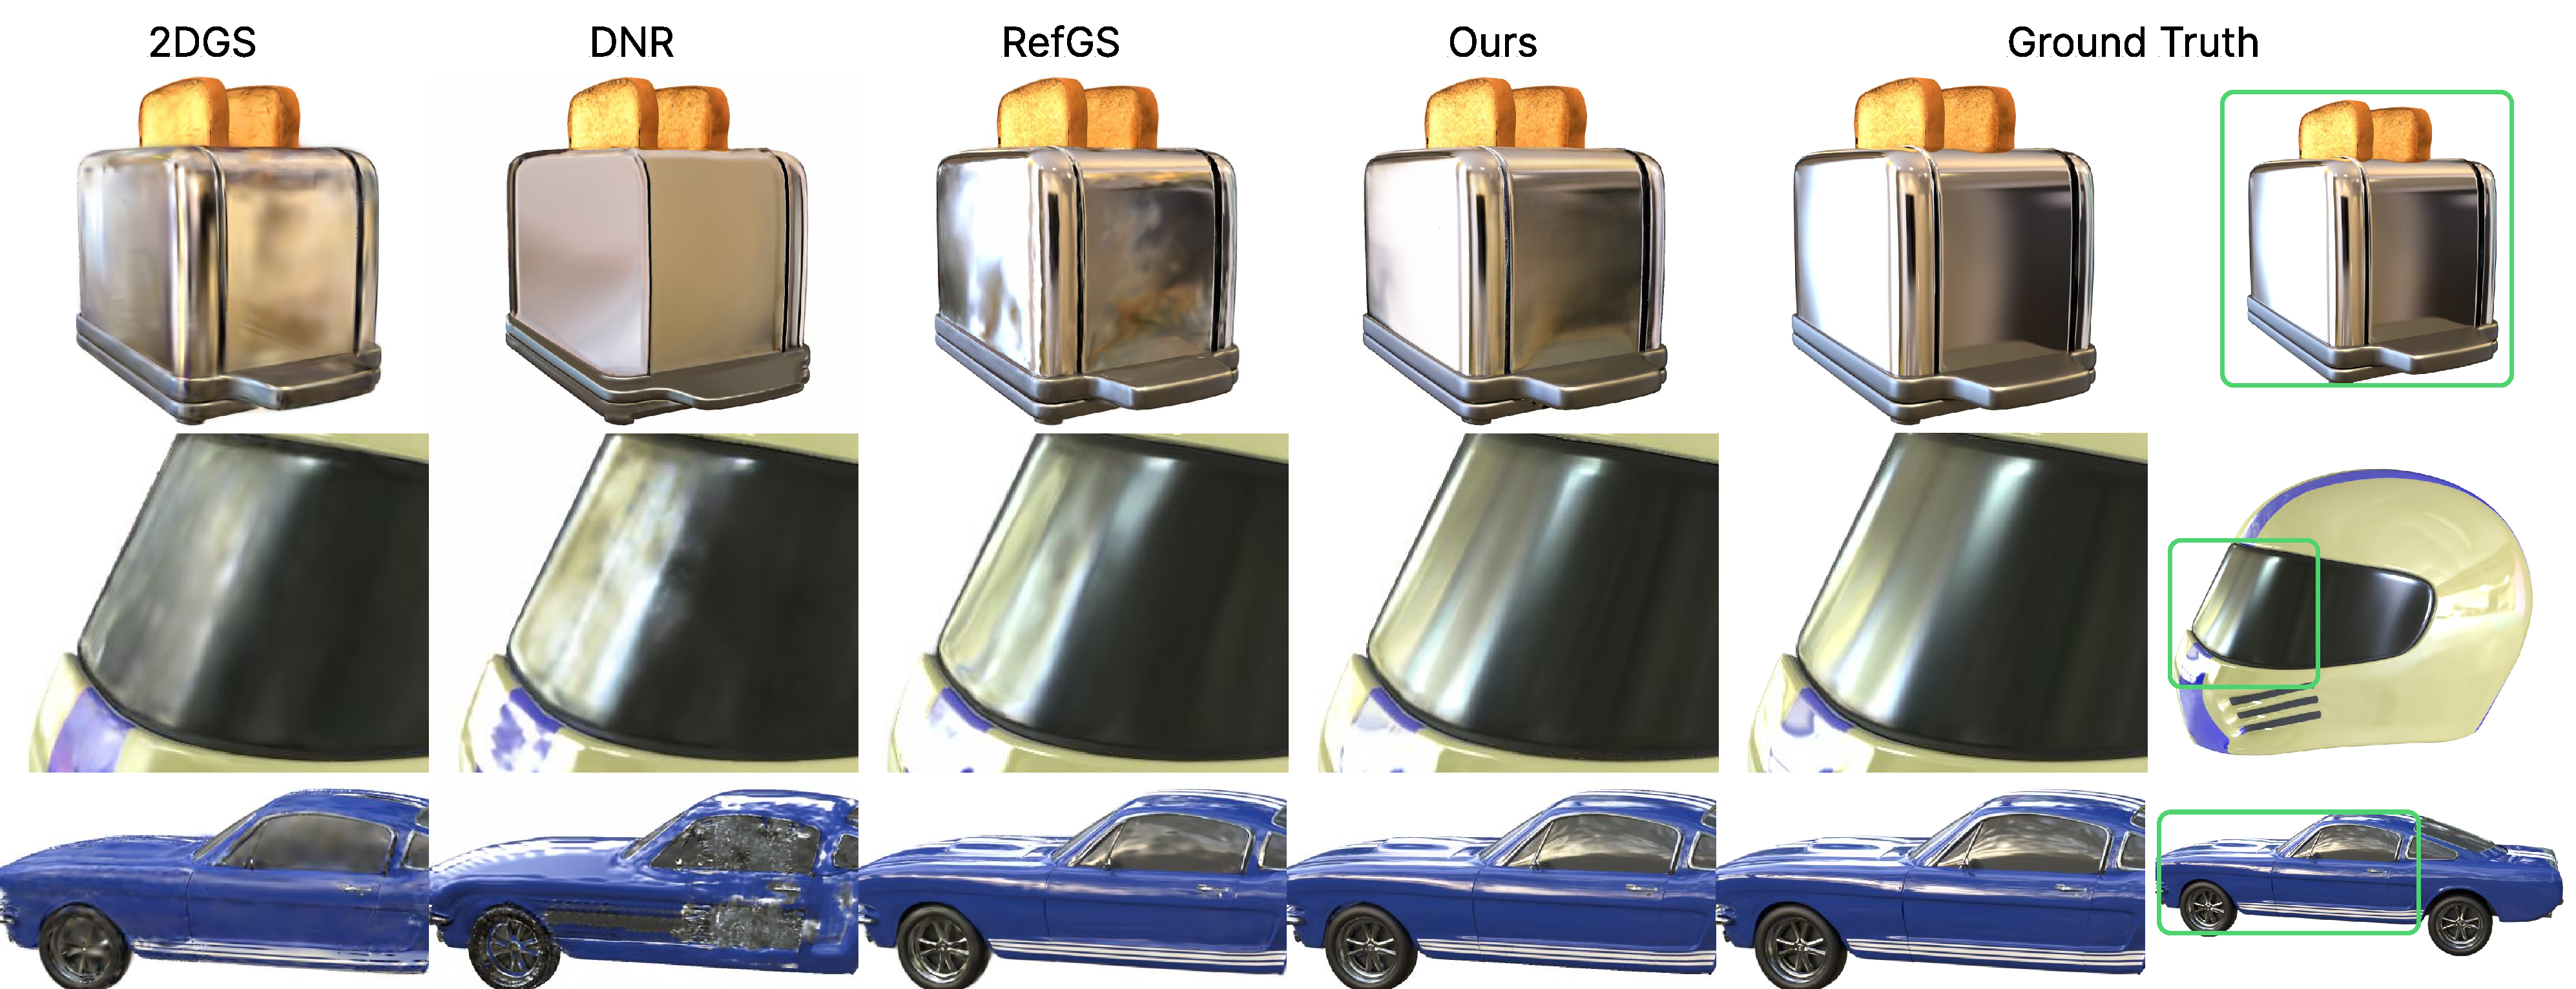
\includegraphics[width=0.95\linewidth]{figs/qualitative.pdf}
    \caption{\textbf{Qualitative comparison on Shiny-Blender.} From left to right: the mesh-constrained baseline 2DGS$^{*}$, DNR, the state-of-the-art RefGS, our method, and ground truth (GT). Our renders reproduce the sharp, high-frequency environment reflections on the metallic surfaces most faithfully; 2DGS$^{*}$ and DNR blur or smear them, RefGS recovers them less crisply.}
    \label{fig:qualitative}
    \vspace{-2mm}
\end{figure}
\paragraph{Growing the maps by error.}
We do not fix the number of maps in advance. Training begins with one map shared by the whole object. Periodically we attribute the current reconstruction error to parts and split off the highest-error \emph{connected} region into a new child map, warm-started by copying its parent. Repeated up to a small budget (five maps in our experiments), this spends capacity where reflection error is largest, isolating the concave pockets a single map cannot explain.

\paragraph{Blending across borders.}
Hard per-face routing would leave visible seams at part boundaries. Instead, each face holds a soft
membership over the maps and a fragment reads \emph{every} map at $\boldsymbol{\omega}_r$:
%
\begin{equation}
E(\boldsymbol{\omega}_r, f) = \sum_{p} \beta_p(f)\, E_p(\boldsymbol{\omega}_r),
\qquad
\beta_p(f) = \operatorname{softmax}_p\!\big(-d_p(f)/\tau\big),
\label{eq:envblend}
\end{equation}
%
where $d_p(f)$ is the distance from face $f$ to the nearest face assigned to map $p$, and $\tau$
sets the blend width: $\beta$ is $\approx$ one-hot inside a region and blends smoothly within
$\sim\tau$ of a border, so the weighted fetch removes the seam. Each $E_p$ stores a learned
multi-channel feature rather than RGB, decoded into reflected color by the network of
Sec.~\ref{sec:kan}.

\subsection{The FastKAN Reflection Decoder}
\label{sec:kan}
The fields of Secs.~\ref{sec:gmm} and~\ref{sec:env} are tied together by a learnable decoder: it
consumes a surface point, its viewing geometry, and the part-blended environment feature, and emits
the view-dependent reflection $r(\mathbf{x},\mathbf{v})$ of Eq.~\eqref{eq:appearance}. The decoder
is interchangeable. We use a Fast Kolmogorov--Arnold Network, which places a learnable activation on
every \emph{edge} rather than a fixed nonlinearity on every node \cite{kan}, realized with Gaussian
radial basis functions on a small fixed grid \cite{fastkan}; on our task it outperforms a
parameter-matched MLP by $1.39$ dB (Sec.~\ref{sec:ablation}). Where inference cost matters more than
fidelity, an MLP or a precomputed lookup table can occupy the same slot.

\paragraph{Staged inputs.}
The decoder is a deferred, staged shader~\citep{refnerf}: view-independent quantities are consumed
before view-dependent ones, with two KAN layers per stage. (1) \emph{Position}: the Fourier
positional encoding of the hit point $\mathbf{x}$ (bounding-box normalized, six frequencies), which
localizes appearance on the surface. (2) \emph{Normal}: the real spherical harmonics
$\mathrm{SH}(\mathbf{n})$ of the surface normal (degree $4$) are appended. (3) \emph{View}: the
integrated directional encoding $\mathrm{IDE}(\boldsymbol{\omega}_r)$ of the reflected direction is
appended together with $\mathbf{n}\!\cdot\!\mathbf{v}$; the IDE is $\mathrm{SH}(\boldsymbol{\omega}_r)$
attenuated by a learned per-point roughness, so a rougher surface queries the environment over a
wider cone --- a prefiltered, glossy lookup rather than a perfect mirror. This stage emits the
material feature $\mathbf{h}$.

\paragraph{Environment fusion and output.}
A two-layer linear MLP fuses $\mathbf{h}$ with the part-blended environment feature
$E(\boldsymbol{\omega}_r,f)$ of Eq.~\eqref{eq:envblend}, and a linear head emits the reflection
$r(\mathbf{x},\mathbf{v})$ of Eq.~\eqref{eq:appearance}, scaled by a learned specular tint in
$[0,1]^3$. Only the staged trunk is KAN. The color head is zero-initialized, so reflection starts at
zero and is turned \emph{up} only where the training views demand it.

\subsection{Downstream Tasks}
\label{sec:downstream}
The baked asset supports two tasks beyond rendering. Both operate on a trained model and leave the
representation of Secs.~\ref{sec:gmm}--\ref{sec:kan} unchanged.
\subsubsection{Mesh Refinement}
\label{sec:refinement}
Anchoring leaves the field blind along the surface normal: the blend weights of Eq.~\eqref{eq:pou}
depend only on in-plane offsets, so a gradient evaluated on the surface vanishes in $\mathbf{n}$. A
disk can ask the mesh to slide, never to move in or out. We recover the missing direction by
detaching the disk centers for a single backward pass and evaluating them in ray-splat
form~\citep{2DGS}, which reads where each disk would move if it were free. That request is then
distributed onto the face's vertices through the same barycentric weights that reconstructed it,
restricted to the vertex normal, band-limited to the disk radius, and capped per cycle. The disks
themselves never leave the surface: they are re-anchored once the vertex update commits, so the
field remains a parameterization of the mesh throughout. Alternating this geometry step with an
ordinary appearance step refines the mesh the asset is baked onto; we evaluate it in
Sec.~\ref{sec:Exp} and give the algorithm in \textcolor{red}{App.~\ref{app:refinement}.}



\begin{table}[t]
\centering
\caption{Quantitative comparison on NeRF Synthetic and Shiny-Blender datasets. Ranking
(\colorbox{green!25}{\textbf{1st}}, \colorbox{orange!25}{2nd}, \colorbox{yellow!25}{3rd}) is
computed within the Fixed-Mesh block only, since these methods share our input mesh; the No-Mesh
and Flexible-Mesh blocks reconstruct their own geometry and are shown as context, not ranked
(numbers reported from RefGS~\citep{refgs}). The Fixed-Mesh rows (2DGS$^{*}$, DNR, and Ours) are
measured by us.}
\label{tab:main}
\resizebox{\linewidth}{!}{
\begin{tabular}{llcccccc}
\toprule
\multirow{2}{*}{\textbf{Constraint}} & \multirow{2}{*}{\textbf{Method}} & \multicolumn{3}{c}{NeRF Synthetic} & \multicolumn{3}{c}{Shiny-Blender} \\
\cmidrule(lr){3-5} \cmidrule(lr){6-8}
& & PSNR$\uparrow$ & SSIM$\uparrow$ & LPIPS$\downarrow$ & PSNR$\uparrow$ & SSIM$\uparrow$ & LPIPS$\downarrow$ \\
\midrule
\multirow{5}{*}{No Mesh (context)}
& Ref-NeRF~\citep{refnerf}     & 31.29 & 0.947 & 0.058 & 32.32 & 0.956 & 0.110 \\
& 3DGS~\citep{3DGS}         & 33.30 & 0.969 & 0.030 & 30.37 & 0.947 & 0.083 \\
& 3iGS~\citep{3igs}         & 33.60 & 0.970 & 0.029 & 30.64 & 0.948 & 0.077 \\
& ENVIDR~\citep{envidr}       & 28.13 & 0.953 & 0.068 & 32.88 & 0.969 & 0.072 \\
& 3DGS-DR~\citep{3dgsDR}      & 31.02 & 0.962 & 0.047 & 33.94 & 0.971 & 0.059 \\
\midrule
\multirow{2}{*}{Flexible Mesh (context)}
& GShader~\citep{gaussianShader}      & 31.48 & 0.960 & 0.042 & 30.42 & 0.951 & 0.082 \\
& RefGS~\citep{refgs}             & 33.20 & 0.966 & 0.036 & 34.80 & 0.973 & 0.056 \\
\midrule
\multirow{2}{*}{Fixed Mesh}
& DNR~\citep{DNR}               & \cellcolor{yellow!25}32.01 & \cellcolor{yellow!25}0.959 & \cellcolor{yellow!25}0.043 & \cellcolor{yellow!25}27.50 & \cellcolor{yellow!25}0.930 & \cellcolor{yellow!25}0.097 \\
& 2DGS*~\citep{2DGS}             & \cellcolor{orange!25}32.32 & \cellcolor{orange!25}0.960 & \cellcolor{green!25}\textbf{0.029} & \cellcolor{orange!25}27.70 & \cellcolor{orange!25}0.931 & \cellcolor{orange!25}0.078 \\
\midrule
Fixed Mesh & Ours              & \cellcolor{green!25}\textbf{33.74} & \cellcolor{green!25}\textbf{0.974} & \cellcolor{orange!25}0.035 & \cellcolor{green!25}\textbf{38.04} & \cellcolor{green!25}\textbf{0.9830} & \cellcolor{green!25}\textbf{0.0238} \\
\bottomrule
\end{tabular}
}
\end{table}

\vspace{-1mm}
\section{Experiments}
\vspace{-1mm}
\label{sec:Exp}
\textbf{Novel View Synthesis} We conduct experiments on NeRF-Synthetic~\citep{NeRFVanilla} and Shiny-Blender~\citep{refnerf} in a \emph{fixed mesh setting}. We choose two fixed-mesh baselines:  DNR~\citep{DNR} and a mesh-constrained 2DGS, denoted
2DGS$^{*}$~\citep{2DGS}. We initialize 2DGS$^{*}$ with four million 2D Gaussians uniformly on the surface
and all gradients are projected onto the manifold defined by the mesh faces. We also report
no-mesh methods (Ref-NeRF~\citep{refnerf}, 3DGS~\citep{3DGS}, 3iGS~\citep{3igs}, ENVIDR~\citep{envidr}, 3DGS-DR~\citep{3dgsDR}) and
flexible-mesh methods (GaussianShader~\citep{gaussianShader}, RefGS~\citep{refgs}) as reference. Note that
these methods optimize geometry rather than taking it as given, so they are not directly comparable.


\subsection{Ordering Degeneracy}
\label{sec:ordering}
Theorem B (App.~\ref{app:theory}) predicts that a fixed normal offset cannot repair the ordering
obstruction of Sec.~\ref{sec:intro}: every finite offset still flips at some visible view, and the
offset itself receives no learning signal. We confirm this on 2DGS$^{*}$: displacing every disk by
a fixed $\varepsilon$ along the face normal at initialization, with no further normal motion during
training, PSNR stays flat from $\varepsilon{=}10^{-5}$ to $10^{-3}$ and matches the tied $\varepsilon{=}0$ baseline
(Table~\ref{tab:ordering}).
\begin{table}[t]
\centering
\caption{\textbf{Ordering degeneracy.} Mean Shiny-Blender PSNR for 2DGS$^{*}$ with a fixed per-disk
normal offset $\varepsilon$ at initialization, versus the tied $\varepsilon{=}0$ baseline
(Table~\ref{tab:combined-ablation-baselines}). PSNR does not improve with $\varepsilon$.}
\label{tab:ordering}
\begin{tabular}{lcccc}
\toprule
Dataset & $\varepsilon{=}0$ (baseline) & $10^{-5}$ & $10^{-4}$ & $10^{-3}$ \\
\midrule
Shiny-Blender (PSNR$\uparrow$) & 27.70 & 27.63 & 27.59 & 27.66 \\
\bottomrule
\end{tabular}
\end{table}


\vspace{-2mm}
\subsection{Appearance Quality}
\label{sec:quality}
Given the mesh, our appearance field reaches $38.04$~dB PSNR on Shiny-Blender and $33.74$~dB on
NeRF-Synthetic (Table~\ref{tab:main}), the best result among fixed-mesh methods that share our
input mesh; the no-mesh and flexible-mesh rows reconstruct their own geometry and are shown as
context, not ranked against ours. The margin over the best context method
(Table~\ref{tab:shiny_perscene}) tracks how reflective a scene is, from $+6.12$~dB on the
near-mirror \emph{ball} down to $+0.45$~dB on \emph{teapot}, whose highlights are smallest.
Qualitatively (Figure~\ref{fig:qualitative}), our renders reproduce sharp, high-frequency
reflections on metallic surfaces that 2DGS$^{*}$ and DNR blur.


\begin{figure}[t]
    \centering
    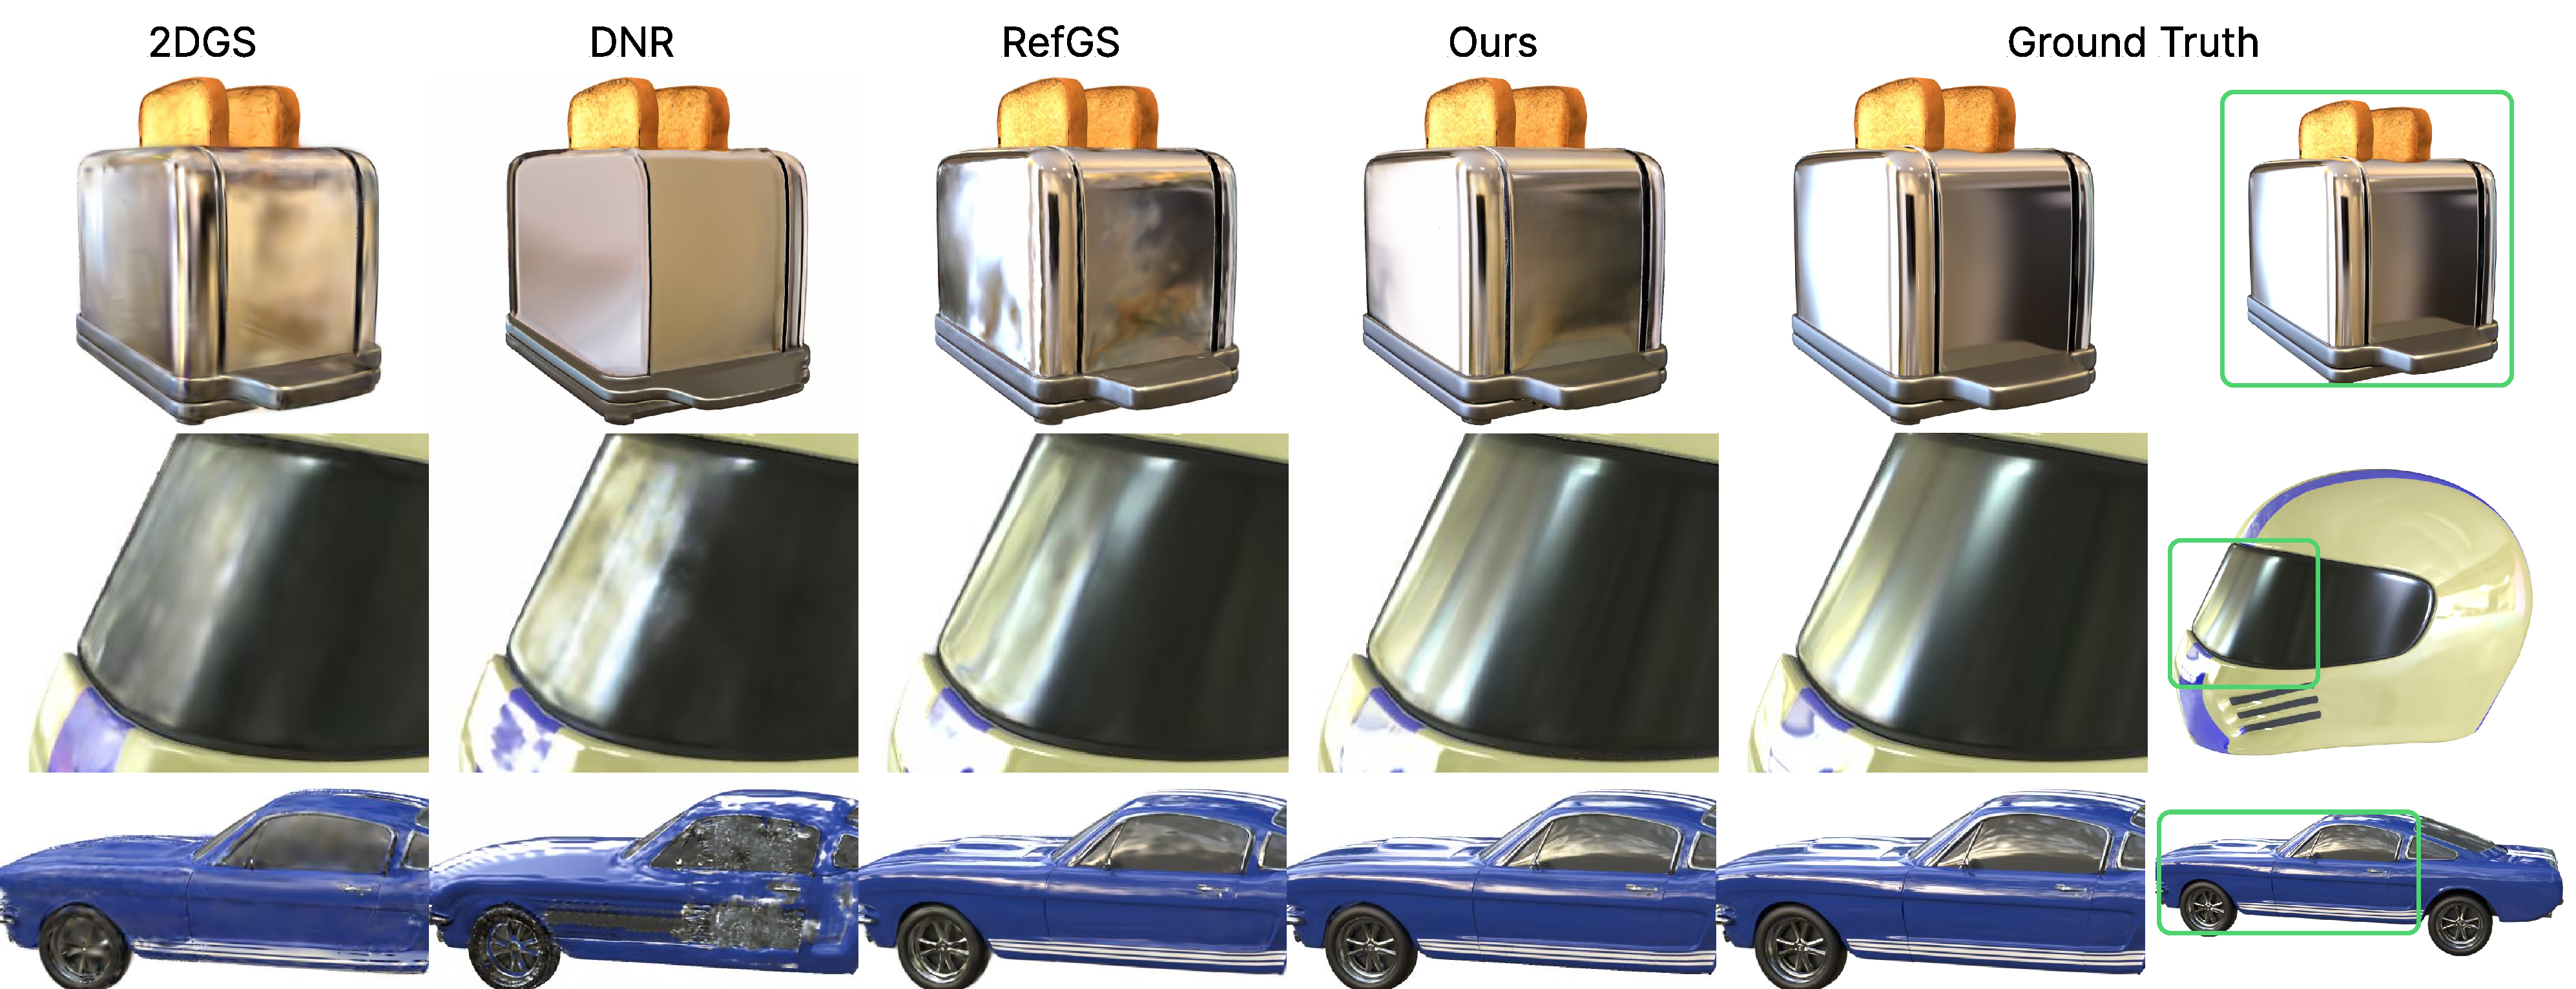
\includegraphics[width=0.95\linewidth]{figs/qualitative.pdf}
    \caption{\textbf{Qualitative comparison on Shiny-Blender.} From left to right: the mesh-constrained baseline 2DGS$^{*}$, DNR, the state-of-the-art RefGS, our method, and ground truth (GT); the rightmost column marks the magnified region on the full object. Our renders reproduce the sharp, high-frequency environment reflections on the metallic surfaces most faithfully; 2DGS$^{*}$ and DNR blur or smear them, RefGS recovers them less crisply.}
    \label{fig:qualitative}
    \vspace{-2mm}
\end{figure}


\subsection{Ablation}
\label{sec:ablation}
Table~\ref{tab:ablation} follows the path by which the appearance model was built. The coplanar
2DGS$^{*}$ baseline suffers the depth-fighting of Sec.~\ref{sec:intro}, and a purely diffuse mixture
cannot represent view-dependent reflection, so both collapse on the reflective scenes. Per-primitive
view-dependent color --- spherical harmonics in 3DGS, or the anisotropic spherical Gaussians of
Spec-Gaussian~\citep{specGaussian} --- is strong for \emph{floating} splats, where overlapping,
depth-ordered primitives compose the appearance. On a single opaque surface that composition is
unavailable: each point takes one order-independent blend, so a per-primitive spherical Gaussian
with an MLP decoder only overfits the sparse views ($34.24$~dB), and dropping it barely changes the
result (Table~\ref{tab:ablation}). The gains come instead from the adaptive hierarchical maps
($+1.2$~dB over a single global map) and from the KAN decoder ($+2.44$~dB over a parameter-matched
MLP).



\subsection{Efficiency}
The full asset ($10^6$ disks, five environment maps, shader) occupies $48.3$ MB on disk. At
$800{\times}800$ we render at $91.7$ FPS on NeRF-Synthetic and $68.6$ FPS on
Shiny-Blender on an NVIDIA H100 (CUDA 12.8), and at $76.8$ FPS on Shiny-Blender on a consumer RTX
4090 (WSL2, Ubuntu 22.04), with a mean CUDA memory footprint of $1.74$ GB (peak $2.75$ GB), all under \texttt{torch.compile}.

% The full asset ($10^6$ disks, five environment maps, shader) occupies $48.3$ MB on disk. At
% $800{\times}800$ we render the test views at $91.7$ FPS on NeRF-Synthetic and $68.6$ FPS on
% Shiny-Blender on an NVIDIA H100 (CUDA 12.8), and at $76.8$ FPS on Shiny-Blender on a consumer RTX
% 4090 (WSL2, Ubuntu 22.04), with a mean CUDA memory footprint of $1.74$ GB (peak $2.75$ GB). All measurements use \texttt{torch.compile}; the H100 figures are from a shared datacenter node.

\subsection{Compaction}
\label{sec:compaction}
Because each disk is an ordinary splat rather than a bespoke primitive, we compact the baked
asset with NanoGS~\citep{nanogs}, a training-free Gaussian-splat simplifier, with no change to our
representation or pipeline. Table~\ref{tab:compaction} reports mean PSNR/SSIM/LPIPS on
Shiny-Blender as we keep 100\%, 50\%, 25\%, and 10\% of the disks: at $10\times$ compaction, mean
PSNR falls by only $2.0$~dB ($38.04\to36.03$), with SSIM and LPIPS degrading similarly gracefully.
Per-scene results (Table~\ref{tab:compaction_perscene}, App.~\ref{app:compaction}) show \emph{teapot} and \emph{ball} essentially unaffected even at $10\times$, while the more detailed \emph{helmet} loses the most. Because compaction reuses tooling built for the Gaussian-splatting community rather than a bespoke method, our representation is compatible with that ecosystem by construction.
\begin{table*}[t]
\centering
\footnotesize
\setlength{\tabcolsep}{3pt}
\begin{minipage}[t]{0.48\textwidth}
\centering
\caption{\textbf{Ablation on Shiny-Blender} along our development path (dataset means;
\textbf{best} in bold). From the 2DGS$^{*}$ baseline we place the mixture on the manifold (2D GMM),
add a per-primitive spherical-Gaussian (SG) reflection with an MLP decoder, drop SG, add our
adaptive hierarchical environment maps (AdaMap), and finally replace the MLP with our KAN. The MLP
and KAN decoders are matched in parameter count.}
\label{tab:ablation}
\begin{tabular}{@{}lccc@{}}
\toprule
Variant & PSNR$\uparrow$ & SSIM$\uparrow$ & LPIPS$\downarrow$ \\
\midrule
2DGS$^{*}$ (baseline) & 27.70 & 0.930 & 0.078 \\
\quad 2D GMM          & 31.40 & 0.952 & 0.057 \\
\quad + SG + MLP      & 34.24 & 0.961 & 0.051 \\
\quad + MLP           & 34.37 & 0.963 & 0.049 \\
\quad + MLP + AdaMap  & 35.60 & 0.971 & 0.038 \\
\quad + KAN + AdaMap  & \textbf{36.99} & \textbf{0.978} & \textbf{0.033} \\
\bottomrule
\end{tabular}
\end{minipage}
\hfill
\begin{minipage}[t]{0.48\textwidth}
\centering
\caption{\textbf{Mesh refinement.} Geometric Metrics Means over the six Shiny-Blender scenes, from Ref-GS
TSDF extractions, without $\rightarrow$ with refinement. MAE$_\text{face}$ refers to face normals of the optimized mesh while MAE$_\text{vert}$  refers to the per-vertex normals of the mesh. We compare against 200 test view normals in ShinyBlender in ray-splat space. Accuracy on a 3d per-point basis with the ground truth mesh is reported. PSNR is a control, not
a result: it confirms the geometry gains are not obtained by trading image quality. These runs use a
single environment map, so absolute PSNR is below Table~\ref{tab:main}. Per-scene results in
App.~\ref{app:refinement}.}
\label{tab:refinement}
% \begin{tabular}{@{}lcc@{}}
% \toprule
% & w/o $\rightarrow$ w/ & $\Delta$ \\
% \midrule
% VN Normal MAE ($^\circ$)$\downarrow$    & $6.31 \rightarrow 5.41$     & $-14.2\%$ \\
% FN MAE ($^\circ$)$\downarrow$    & $7.20 \rightarrow 5.88$     & $-18.3\%$ \\
% CD $\downarrow$                  & $16.200 \rightarrow 15.889$ & $-2.3\%$  \\
% \midrule
% PSNR $\uparrow$ \emph{(control)} & $27.41 \rightarrow 27.86$   & $+0.45$ db   \\
% \bottomrule
% \end{tabular}
\begin{tabular}{@{}lcc@{}}
\toprule
& w/o $\rightarrow$ w/ & Improvement \\
\midrule
MAE$_\text{face}$ ($^\circ$)$\downarrow$ & $7.20 \rightarrow 5.88$ & $+18.3\%$ \\
MAE$_\text{vert}$ ($^\circ$)$\downarrow$ & $6.31 \rightarrow 5.41$ & $+14.2\%$ \\
Acc.\ ($\times10^{-3}$)$\downarrow$      & $5.80 \rightarrow 5.47$ & $+5.7\%$  \\
\midrule
PSNR (dB)$\uparrow$ \emph{(control)}     & $27.41 \rightarrow 27.86$ & $+0.45$ \\
\bottomrule
\end{tabular}

\end{minipage}
\vspace{-2mm}
\end{table*}
\section{Conclusion and Discussion}
\label{sec:conclusion}
We present automatic neural baking, the first differentiable method to optimize view-dependent appearance as an element-wise ``texture'' on a 2D manifold representation. This enables real-time evaluation (over 60 FPS) directly within the fragment shader of traditional rendering pipelines. Our framework introduces three configurable modules: (1) a 2D kernel, specifically a 2D Gaussian Mixture, to model diffuse color; (2) an adaptive environment map to capture specular reflections; and (3) a neural shader that smoothly interpolates the sparse color representation. Furthermore, our approach surpasses current state-of-the-art methods on standard novel view synthesis benchmarks.

Anisotropic spherical Gaussians (ASG) are a strong per-primitive appearance model~\citep{specGaussian}. In our on-manifold setting, however, such a per-primitive term must be fit from images alone, so it overfits the sparse training views (Table~\ref{tab:ablation}). When the mesh already carries material properties, the ASG parameters can instead be read directly from the mesh rather than optimized from sparse views, which removes this overfitting. This direction is orthogonal to our on-manifold baking formulation, so we regard it as promising future work rather than a limitation.


\bibliography{references}
\bibliographystyle{iclr2027_conference}
\newpage
\appendix
\section{Appendix}
\subsection{Ablation Details}

Here, we present detailed qualitative and quantitative results from our ablation study comparing our approach against closely related baselines. We first evaluated replacing the KAN with a standard MLP. Additionally, we experimented with incorporating material tokens or features, similar to scaffolded Gaussian Splats; however, the performance was inferior to that of a straightforward MLP. We also attempted to use spherical Gaussians for the view-dependent representation, but this approach yielded suboptimal results. These quantitative comparisons are summarized in Tab.~\ref{tab:combined-ablation-baselines}.

Furthermore, we provide qualitative visualizations that decompose the outputs of our method. Specifically, our rendering function consists of three components: multiple environment maps for self-reflection, a KAN for specular reflection, and a GMM for diffuse lighting. We visualize the distinct contributions of each of these lighting components. To isolate the effects of the 2D GMM, Fig.~\ref{fig:abl_qualitative} compares our method against a 2DGS baseline exhibiting depth-fighting (with spherical harmonics set to zero). Finally, Tab.~\ref{tab:shiny_perscene} details a per-scene comparison against reported state-of-the-art results on the Shiny-Blender dataset; these methods reconstruct their own geometry rather than being given ours, so, following Table~\ref{tab:main}, they are shown as context rather than ranked.

% Auto-generated ablation tables (8 = 2 datasets x 4 variants)
% metrics: PSNR (dB, higher better), SSIM (higher), LPIPS (lower)
% Auto-generated ablation tables (8 = 2 datasets x 4 variants)
% metrics: PSNR (dB, higher better), SSIM (higher), LPIPS (lower)
\begin{table}[t]
  \centering
  \caption{Ablation comparisons across all datasets and scenes. Ranking
  (\colorbox{green!25}{\textbf{1st}}, \colorbox{orange!25}{2nd}, \colorbox{yellow!25}{3rd}) is
  restricted to Ours, DNR, and 2DGS$^{*}$, the fixed-mesh methods that share our input mesh
  (following Table~\ref{tab:main}); the ablation-variant columns are not ranked, since they trace
  an internal progression rather than a competing baseline.}
  \label{tab:combined-ablation-baselines}
  \resizebox{\linewidth}{!}{
  \begin{tabular}{llccccccc}
    \toprule
    \multirow{2}{*}{Dataset} & \multirow{2}{*}{Scene} & \multicolumn{5}{c}{Ablation Variants} & \multicolumn{2}{c}{Fixed-mesh baselines} \\
    \cmidrule(lr){3-7} \cmidrule(lr){8-9}
    & & MLP+SG+M Token & MLP + M Token & MLP & 1-Env MLP & Ours & DNR & 2DGS$^{*}$ \\
    \midrule
    \multicolumn{9}{c}{\textbf{PSNR$\uparrow$}} \\
    \midrule
    \multirow{9}{*}{\rotatebox{90}{{NeRF-Synthetic}}}
    & Chair     & 33.43 & 31.30 & 33.22 & 33.45 & \cellcolor{orange!25} 33.00 & \cellcolor{yellow!25} 31.91 & \cellcolor{green!25} \textbf{33.63} \\
    & Drums     & 27.16 & 26.98 & 26.97 & 27.42 & \cellcolor{green!25} \textbf{27.81} & \cellcolor{yellow!25} 25.11 & \cellcolor{orange!25} 25.90 \\
    & Ficus     & 32.45 & 32.43 & 32.48 & 32.66 & \cellcolor{yellow!25} 32.94 & \cellcolor{green!25} \textbf{35.42} & \cellcolor{orange!25} 33.73 \\
    & Hotdog    & 37.15 & 36.74 & 37.03 & 37.13 & \cellcolor{green!25} \textbf{37.60} & \cellcolor{orange!25} 37.43 & \cellcolor{yellow!25} 36.53 \\
    & Lego      & 35.47 & 34.98 & 35.45 & 35.54 & \cellcolor{green!25} \textbf{36.14} & \cellcolor{yellow!25} 34.11 & \cellcolor{orange!25} 34.46 \\
    & Materials & 32.24 & 32.48 & 32.25 & 32.26 & \cellcolor{green!25} \textbf{34.58} & \cellcolor{orange!25} 28.83 & \cellcolor{yellow!25} 27.34 \\
    & Mic       & 35.12 & 35.64 & 35.09 & 35.41 & \cellcolor{green!25} \textbf{36.66} & \cellcolor{yellow!25} 34.89 & \cellcolor{orange!25} 35.96 \\
    & Ship      & 30.28 & 30.56 & 30.27 & 30.66 & \cellcolor{green!25} \textbf{31.18} & \cellcolor{yellow!25} 28.41 & \cellcolor{orange!25} 31.02 \\
    \cmidrule{2-9}
    & \textbf{Mean} & 32.91 & 32.64 & 32.84 & 33.07 & \cellcolor{green!25} \textbf{33.74} & \cellcolor{yellow!25} 32.01 & \cellcolor{orange!25} 32.32 \\
    \midrule
    \multirow{7}{*}{\rotatebox{90}{Shiny-Blender}}
    & Ball      & 40.32 & 43.90 & 39.74 & 40.38 & \cellcolor{green!25} \textbf{45.01} & \cellcolor{orange!25} 21.83 & \cellcolor{yellow!25} 20.99 \\
    & Car       & 28.07 & 29.49 & 28.18 & 29.50 & \cellcolor{green!25} \textbf{33.75} & \cellcolor{yellow!25} 21.11 & \cellcolor{orange!25} 26.41 \\
    & Coffee    & 33.47 & 34.28 & 33.28 & 32.85 & \cellcolor{green!25} \textbf{35.33} & \cellcolor{yellow!25} 31.04 & \cellcolor{orange!25} 32.26 \\
    & Helmet    & 34.19 & 35.82 & 34.27 & 34.16 & \cellcolor{green!25} \textbf{37.94} & \cellcolor{orange!25} 26.82 & \cellcolor{yellow!25} 26.23 \\
    & Teapot    & 44.72 & 46.96 & 44.18 & 44.40 & \cellcolor{green!25} \textbf{47.45} & \cellcolor{orange!25} 43.60 & \cellcolor{yellow!25} 40.75 \\
    & Toaster   & 24.66 & 23.15 & 24.25 & 24.92 & \cellcolor{green!25} \textbf{28.76} & \cellcolor{orange!25} 20.58 & \cellcolor{yellow!25} 19.55 \\
    \cmidrule{2-9}
    & \textbf{Mean} & 34.24 & 35.60 & 33.98 & 34.37 & \cellcolor{green!25} \textbf{38.04} & \cellcolor{yellow!25} 27.50 & \cellcolor{orange!25} 27.70 \\

    \midrule
    \multicolumn{9}{c}{\textbf{SSIM$\uparrow$}} \\
    \midrule
    \multirow{9}{*}{\rotatebox{90}{{NeRF-Synthetic}}}
    & Chair     & 0.9797 & 0.9682 & 0.9790 & 0.9797 & \cellcolor{orange!25} 0.9767 & \cellcolor{yellow!25} 0.9747 & \cellcolor{green!25} \textbf{0.9808} \\
    & Drums     & 0.9558 & 0.9583 & 0.9545 & 0.9572 & \cellcolor{green!25} \textbf{0.9629} & \cellcolor{yellow!25} 0.9427 & \cellcolor{orange!25} 0.9502 \\
    & Ficus     & 0.9772 & 0.9777 & 0.9773 & 0.9782 & \cellcolor{yellow!25} 0.9800 & \cellcolor{green!25} \textbf{0.9848} & \cellcolor{orange!25} 0.9820 \\
    & Hotdog    & 0.9849 & 0.9848 & 0.9845 & 0.9848 & \cellcolor{green!25} \textbf{0.9869} & \cellcolor{orange!25} 0.9859 & \cellcolor{yellow!25} 0.9826 \\
    & Lego      & 0.9812 & 0.9808 & 0.9812 & 0.9814 & \cellcolor{green!25} \textbf{0.9836} & \cellcolor{yellow!25} 0.9764 & \cellcolor{orange!25} 0.9765 \\
    & Materials & 0.9670 & 0.9733 & 0.9671 & 0.9671 & \cellcolor{green!25} \textbf{0.9812} & \cellcolor{orange!25} 0.9523 & \cellcolor{yellow!25} 0.9193 \\
    & Mic       & 0.9884 & 0.9896 & 0.9883 & 0.9894 & \cellcolor{green!25} \textbf{0.9918} & \cellcolor{yellow!25} 0.9861 & \cellcolor{orange!25} 0.9892 \\
    & Ship      & 0.8941 & 0.9091 & 0.8943 & 0.9023 & \cellcolor{green!25} \textbf{0.9145} & \cellcolor{yellow!25} 0.8688 & \cellcolor{orange!25} 0.8995 \\
    \cmidrule{2-9}
    & \textbf{Mean} & 0.9660 & 0.9677 & 0.9658 & 0.9675 & \cellcolor{green!25} \textbf{0.9722} & \cellcolor{yellow!25} 0.9590 & \cellcolor{orange!25} 0.9600 \\
    \midrule
    \multirow{7}{*}{\rotatebox{90}{Shiny-Blender}}
    & Ball      & 0.9847 & 0.9935 & 0.9837 & 0.9848 & \cellcolor{green!25} \textbf{0.9945} & \cellcolor{orange!25} 0.9075 & \cellcolor{yellow!25} 0.8860 \\
    & Car       & 0.9320 & 0.9453 & 0.9322 & 0.9384 & \cellcolor{green!25} \textbf{0.9763} & \cellcolor{yellow!25} 0.8835 & \cellcolor{orange!25} 0.9207 \\
    & Coffee    & 0.9669 & 0.9754 & 0.9660 & 0.9682 & \cellcolor{green!25} \textbf{0.9777} & \cellcolor{yellow!25} 0.9662 & \cellcolor{orange!25} 0.9672 \\
    & Helmet    & 0.9759 & 0.9868 & 0.9763 & 0.9760 & \cellcolor{green!25} \textbf{0.9902} & \cellcolor{orange!25} 0.9525 & \cellcolor{yellow!25} 0.9403 \\
    & Teapot    & 0.9963 & 0.9979 & 0.9959 & 0.9960 & \cellcolor{green!25} \textbf{0.9983} & \cellcolor{orange!25} 0.9961 & \cellcolor{yellow!25} 0.9942 \\
    & Toaster   & 0.9113 & 0.9262 & 0.9037 & 0.9165 & \cellcolor{green!25} \textbf{0.9607} & \cellcolor{orange!25} 0.8812 & \cellcolor{yellow!25} 0.8736 \\
    \cmidrule{2-9}
    & \textbf{Mean} & 0.9612 & 0.9708 & 0.9596 & 0.9633 & \cellcolor{green!25} \textbf{0.9830} & \cellcolor{orange!25} 0.9312 & \cellcolor{yellow!25} 0.9303 \\

    \midrule
    \multicolumn{9}{c}{\textbf{LPIPS$\downarrow$}} \\
    \midrule
    \multirow{9}{*}{\rotatebox{90}{{NeRF-Synthetic}}}
    & Chair     & 0.0167 & 0.0255 & 0.0176 & 0.0168 & \cellcolor{yellow!25} 0.0197 & \cellcolor{orange!25} 0.0186 & \cellcolor{green!25} \textbf{0.0119} \\
    & Drums     & 0.0388 & 0.0416 & 0.0402 & 0.0376 & \cellcolor{green!25} \textbf{0.0361} & \cellcolor{yellow!25} 0.0547 & \cellcolor{orange!25} 0.0451 \\
    & Ficus     & 0.0307 & 0.0302 & 0.0306 & 0.0302 & \cellcolor{yellow!25} 0.0278 & \cellcolor{green!25} \textbf{0.0109} & \cellcolor{orange!25} 0.0126 \\
    & Hotdog    & 0.0144 & 0.0151 & 0.0150 & 0.0146 & \cellcolor{yellow!25} 0.0130 & \cellcolor{green!25} \textbf{0.0110} & \cellcolor{orange!25} 0.0127 \\
    & Lego      & 0.0112 & 0.0119 & 0.0112 & 0.0108 & \cellcolor{green!25} \textbf{0.0095} & \cellcolor{yellow!25} 0.0153 & \cellcolor{orange!25} 0.0146 \\
    & Materials & 0.0245 & 0.0213 & 0.0245 & 0.0243 & \cellcolor{green!25} \textbf{0.0138} & \cellcolor{orange!25} 0.0446 & \cellcolor{yellow!25} 0.0532 \\
    & Mic       & 0.0179 & 0.0131 & 0.0179 & 0.0165 & \cellcolor{orange!25} 0.0097 & \cellcolor{yellow!25} 0.0189 & \cellcolor{green!25} \textbf{0.0091} \\
    & Ship      & 0.0758 & 0.0793 & 0.0760 & 0.0728 & \cellcolor{green!25} \textbf{0.0691} & \cellcolor{yellow!25} 0.1669 & \cellcolor{orange!25} 0.0751 \\
    \cmidrule{2-9}
    & \textbf{Mean} & 0.0288 & 0.0297 & 0.0291 & 0.0279 & \cellcolor{green!25} \textbf{0.0248} & \cellcolor{yellow!25} 0.0426 & \cellcolor{orange!25} 0.0293 \\
    \midrule
    \multirow{7}{*}{\rotatebox{90}{Shiny-Blender}}
    & Ball      & 0.0496 & 0.0248 & 0.0540 & 0.0490 & \cellcolor{green!25} \textbf{0.0224} & \cellcolor{yellow!25} 0.1848 & \cellcolor{orange!25} 0.1651 \\
    & Car       & 0.0432 & 0.0340 & 0.0428 & 0.0387 & \cellcolor{green!25} \textbf{0.0154} & \cellcolor{yellow!25} 0.1120 & \cellcolor{orange!25} 0.0418 \\
    & Coffee    & 0.0506 & 0.0470 & 0.0525 & 0.0504 & \cellcolor{green!25} \textbf{0.0427} & \cellcolor{yellow!25} 0.0681 & \cellcolor{orange!25} 0.0442 \\
    & Helmet    & 0.0350 & 0.0181 & 0.0347 & 0.0346 & \cellcolor{green!25} \textbf{0.0130} & \cellcolor{orange!25} 0.0617 & \cellcolor{yellow!25} 0.0724 \\
    & Teapot    & 0.0080 & 0.0049 & 0.0085 & 0.0085 & \cellcolor{green!25} \textbf{0.0039} & \cellcolor{orange!25} 0.0052 & \cellcolor{yellow!25} 0.0083 \\
    & Toaster   & 0.1201 & 0.0975 & 0.1324 & 0.1148 & \cellcolor{green!25} \textbf{0.0455} & \cellcolor{yellow!25} 0.1503 & \cellcolor{orange!25} 0.1380 \\
    \cmidrule{2-9}
    & \textbf{Mean} & 0.0511 & 0.0377 & 0.0541 & 0.0493 & \cellcolor{green!25} \textbf{0.0238} & \cellcolor{yellow!25} 0.0970 & \cellcolor{orange!25} 0.0783 \\
    \bottomrule
  \end{tabular}
  }
\end{table}

\begin{table}[t]
  \centering
  \caption{Per-scene comparison on Shiny-Blender against reported results for methods that
  reconstruct their own geometry. Following Table~\ref{tab:main}, these are not given our input
  mesh, so they are shown as context rather than ranked against \textbf{Ours}, which is bolded
  for reference only.}
  \label{tab:shiny_perscene}
  \resizebox{\linewidth}{!}{
  \begin{tabular}{lccccccc}
    \toprule
    & \multicolumn{7}{c}{Shiny-Blender} \\
    & Car & Ball & Helmet & Teapot & Toaster & Coffee & Avg. \\
    \midrule
    \multicolumn{8}{c}{PSNR$\uparrow$} \\
    \midrule
    Ref-NeRF~\citep{refnerf} &  30.41 & 29.14 & 29.92 & 45.19 & 25.29 & 33.99 & 32.32 \\
    NeRO~\citep{nero} & 25.53 & 30.26 & 29.20 & 38.70 & 26.46 & 28.89 & 29.84 \\
    ENVIDR~\citep{envidr} & 28.46 & 38.89 & 32.73 & 41.59 & 26.11 & 29.48 & 32.88 \\
    3DGS~\citep{3DGS} & 27.24 & 27.69 & 28.32 & 45.68 & 20.99 & 32.32 & 30.37 \\
    GaussianShader~\citep{gaussianShader} & 27.51 & 29.02 & 28.73 & 43.05 & 22.86 & 31.34 & 30.42 \\
    3iGS~\citep{3igs} & 27.52 & 26.82 & 28.08 & 46.05 & 22.71 & 32.64 & 30.64 \\
    3DGS-DR~\citep{3dgsDR} & 30.43 & 33.44 & 31.49 & 47.00 & 26.69 & 34.61 & 33.94 \\
    RefGS~\citep{refgs}                & 30.94 & 36.10 & 33.40 & 46.69 & 27.28 & 34.38 & 34.80 \\
    \midrule
    \textbf{Ours}     &  \textbf{33.75} & \textbf{45.01} & \textbf{37.94} & \textbf{47.45} & \textbf{28.76} & \textbf{35.33} & \textbf{38.04} \\
    \midrule
    \multicolumn{8}{c}{SSIM$\uparrow$} \\
    \midrule
    Ref-NeRF~\citep{refnerf} & 0.949 & 0.956 & 0.955 & 0.995 & 0.910 & 0.972 & 0.956 \\
    NeRO~\citep{nero} & 0.949 & 0.974 & 0.971 & 0.995 & 0.929 & 0.956 & 0.962 \\
    ENVIDR~\citep{envidr} & 0.961 & 0.991 & 0.980 & 0.996 & 0.939 & 0.949 & 0.969 \\
    3DGS~\citep{3DGS} & 0.930 & 0.937 & 0.951 & 0.996 & 0.895 & 0.971 & 0.947 \\
    GaussianShader~\citep{gaussianShader} & 0.930 & 0.954 & 0.955 & 0.996 & 0.900 & 0.969 & 0.951 \\
    3iGS~\citep{3igs} & 0.930 & 0.933 & 0.951 & 0.996 & 0.909 & 0.972 & 0.948 \\
    3DGS-DR~\citep{3dgsDR} & 0.962 & 0.979 & 0.971 & 0.997 & 0.942 & 0.976 & 0.971 \\
    RefGS~\citep{refgs}               & 0.961 & 0.981 & 0.975 & 0.997 & 0.942 & 0.973 & 0.973 \\
    \midrule
    \textbf{Ours}            & \textbf{0.9763} & \textbf{0.9945} & \textbf{0.9902} & \textbf{0.9983} & \textbf{0.9607} & \textbf{0.9777} & \textbf{0.9830} \\
    \midrule
    \multicolumn{8}{c}{LPIPS$\downarrow$} \\
    \midrule
    Ref-NeRF~\citep{refnerf} & 0.051 & 0.307 & 0.087 & 0.013 & 0.118 & 0.082 & 0.110 \\
    NeRO~\citep{nero} & 0.074 & 0.094 & 0.050 & 0.012 & 0.089 & 0.110 & 0.072 \\
    ENVIDR~\citep{envidr} & 0.049 & 0.067 & 0.051 & 0.011 & 0.116 & 0.139 & 0.072 \\
    3DGS~\citep{3DGS} & 0.047 & 0.161 & 0.079 & 0.007 & 0.126 & 0.078 & 0.083 \\
    GaussianShader~\citep{gaussianShader} & 0.045 & 0.148 & 0.088 & 0.012 & 0.111 & 0.085 & 0.082 \\
    3iGS~\citep{3igs} & 0.045 & 0.166 & 0.073 & 0.006 & 0.098 & 0.077 & 0.077 \\
    3DGS-DR~\citep{3dgsDR} & 0.034 & 0.104 & 0.050 & 0.006 & 0.083 & 0.076 & 0.059 \\
    RefGS~\citep{refgs}                & 0.034 & 0.098 & 0.045 & 0.006 & 0.070 & 0.082 & 0.056 \\
    \midrule
    \textbf{Ours}     & \textbf{0.0154} & \textbf{0.0224} & \textbf{0.0130} & \textbf{0.0039} & \textbf{0.0455} & \textbf{0.0427} & \textbf{0.0238} \\
    \bottomrule
  \end{tabular}
  }
\end{table}



\begin{figure}
    \centering
    \includegraphics[width=\linewidth]{figs/ablation.pdf}
    \caption{From left to right: 2DGS baseline, 2D GMM for diffuse light, KAN with one environment map, KAN with multiple environment maps, and ground truth. We highlight that our multi-environment setting successfully approximates the self-reflection effects on concave objects in toaster. For convex-objects, since there is nearly no self-reflection, the visual results seems highly aligned}
    \label{fig:abl_qualitative}
\end{figure}

\subsection{Mesh Refinement Through the Anchoring}
\label{app:refinement}
Because each disk center is a barycentric combination of its face's vertices
(Eq.~\eqref{eq:center}), the anchoring is linear in the mesh, $\mathbf{X}=\mathbf{B}\mathbf{V}$, and
photometric gradients reach the vertices. We use this to refine an imperfect input mesh (here, one
extracted from Ref-GS's unconstrained Gaussians), as a demonstration of the property rather than as
a new refinement method: the photometric gradient is taken at the disk centers, evaluated at the
ray--disk intersection, and pulled back to the vertices through the anchoring, similar in spirit to
the mesh-anchored refinement of SuGaR~\citep{sugar} and OMeGa~\citep{omega}; connectivity is fixed.

\paragraph{Setup.} We start from the Ref-GS~\citep{refgs} mesh (TSDF fusion and marching cubes,
then simplification and hole filling), warm up the appearance model on it for 625 optimizer steps,
and freeze the KAN shader and environment maps. We then alternate 300 cycles of a geometry step
(8 training views, one vertex update restricted to the vertex normal, smoothed to $2.5\sigma$ and
capped at $0.5\sigma$ per cycle, $\sigma$ the disk radius) and an appearance step (40 steps on the
disks, mesh fixed). The optional prior is an area-weighted normal-consistency term pulling each face
normal toward the input's shading normals, weighted at half the photometric gradient's norm.
Geometry is scored against the ground-truth Blender models. Normals are scored by mean angular
error against the ground-truth normal maps of the 200 test views. For position, we use the standard
DTU metrics~\citep{dtu}, but report only accuracy (Acc.), the mean distance from points on the
refined mesh to the nearest ground-truth surface visible from the test cameras (lower is better).
Following Ref-NeuS~\citep{ref-neus}, we omit completeness, which is dominated by regions missing
from the input mesh that a fixed-connectivity refinement cannot fill.

\paragraph{Results.} Table~\ref{tab:refine_improve} summarizes the effect of refinement on the
input mesh, and Table~\ref{tab:refine_decomp} separates the two signals.
The prior alone reorients faces toward the smooth shading normals, giving the lowest face-normal
error, but it does not use the images and moves the surface away from the ground truth (accuracy
worsens from $5.83$ to $6.18$). The photometric gradient alone is not enough either: without the
prior, face normals degrade ($7.20^\circ \rightarrow 18.58^\circ$). Together they give the best
vertex-normal error ($6.31^\circ \rightarrow 5.41^\circ$) and accuracy ($5.83 \rightarrow 5.49$).
Figure~\ref{fig:mesh_ringing} shows the effect of refinement on high-frequency surface artifacts
left by the extraction: the fine noise on \emph{teapot} and the concentric marching-cubes ringing
on \emph{helmet} are both smoothed away.

\paragraph{Limitations.} The refinement adjusts an existing surface and cannot recover absent
geometry, starts from a short warm-up rather than a fully trained model, and is not compared
against full reconstruction pipelines such as OMeGa or Ref-NeuS, which also change topology or
reconstruct geometry from scratch.

\begin{table}[t]
\centering
\small
\begin{minipage}[t]{0.40\textwidth}
\centering
\caption{\textbf{Effect of refinement on the input mesh} (means over the six Shiny-Blender scenes),
without $\rightarrow$ with refinement (photometric + normal). Improvement is the relative reduction in
error. Metrics as in Table~\ref{tab:refine_decomp}.}
\label{tab:refine_improve}
\setlength{\tabcolsep}{4pt}
\begin{tabular}{@{}lcc@{}}
\toprule
& w/o $\rightarrow$ w/ & Improvement \\
\midrule
$\mathrm{MAE}_{\mathbf{n}_f}$ ($^\circ$)$\downarrow$ & $7.20 \rightarrow 5.88$ & $+18.3\%$ \\
$\mathrm{MAE}_{\mathbf{n}_v}$ ($^\circ$)$\downarrow$ & $6.31 \rightarrow 5.41$ & $+14.2\%$ \\
Acc.\ ($\times10^{-3}$)$\downarrow$         & $5.83 \rightarrow 5.49$ & $+5.8\%$  \\
\bottomrule
\end{tabular}
\end{minipage}
\hfill
\begin{minipage}[t]{0.56\textwidth}
\centering
\caption{\textbf{Where the refinement gain comes from} (means over the six Shiny-Blender scenes,
lower is better; angular errors in degrees, Acc.\ $\times10^{-3}$). Rows name the terms
optimized: the photometric loss, the normal-consistency prior, or both. Per-scene values in
Table~\ref{tab:refine_perscene}.}
\label{tab:refine_decomp}
\setlength{\tabcolsep}{4pt}
\begin{tabular}{@{}lccc@{}}
\toprule
& $\mathrm{MAE}_{\mathbf{n}_f}\downarrow$ & $\mathrm{MAE}_{\mathbf{n}_v}\downarrow$ & Acc.$\downarrow$ \\
\midrule
Input mesh & 7.20 & 6.31 & 5.83 \\
\midrule
Normal only & \textbf{5.55} & 5.88 & 6.18 \\
Photometric only & 18.58 & 6.53 & 6.11 \\
Photometric + normal & 5.88 & \textbf{5.41} & \textbf{5.49} \\
\bottomrule
\end{tabular}
\end{minipage}
\end{table}

\begin{table}[t]
\centering
\footnotesize
\setlength{\tabcolsep}{3pt}
\caption{\textbf{Per-scene refinement results}, same arms and metrics as
Table~\ref{tab:refine_decomp}. Avg.\ averages the per-scene values. \colorbox{green!25}{\textbf{1st}}, \colorbox{orange!25}{2nd}, and \colorbox{yellow!25}{3rd} best per column are highlighted.}
\label{tab:refine_perscene}
\begin{tabular}{@{}lccccccc@{}}
\toprule
& Helmet & Teapot & Toaster & Coffee & Car & Ball & Avg. \\
\midrule
\multicolumn{8}{c}{MAE$_{\mathbf{n}_f}$ ($^\circ$)$\downarrow$} \\
\midrule
Input mesh & \cellcolor{yellow!25} 4.48 & \cellcolor{yellow!25} 7.25 & \cellcolor{yellow!25} 9.40 & \cellcolor{yellow!25} 9.02 & \cellcolor{yellow!25} 9.81 & \cellcolor{yellow!25} 3.21 & \cellcolor{yellow!25} 7.20 \\
Prior only & \cellcolor{green!25} \textbf{1.98} & \cellcolor{orange!25} 4.99 & \cellcolor{orange!25} 8.45 & \cellcolor{orange!25} 8.85 & \cellcolor{green!25} \textbf{8.41} & \cellcolor{green!25} \textbf{0.62} & \cellcolor{green!25} \textbf{5.55} \\
Ours (image only) & 21.42 & 13.16 & 21.51 & 16.31 & 17.53 & 21.54 & 18.58 \\
Ours (image + prior) & \cellcolor{orange!25} 2.41 & \cellcolor{green!25} \textbf{4.71} & \cellcolor{green!25} \textbf{7.85} & \cellcolor{green!25} \textbf{8.21} & \cellcolor{orange!25} 9.09 & \cellcolor{orange!25} 3.01 & \cellcolor{orange!25} 5.88 \\
\midrule
\multicolumn{8}{c}{MAE$_{\mathbf{n}_v}$ ($^\circ$)$\downarrow$} \\
\midrule
Input mesh & 2.77 & 6.69 & \cellcolor{orange!25} 9.02 & \cellcolor{yellow!25} 10.02 & \cellcolor{yellow!25} 8.69 & \cellcolor{yellow!25} 0.64 & \cellcolor{yellow!25} 6.31 \\
Prior only & \cellcolor{orange!25} 2.61 & \cellcolor{orange!25} 5.52 & \cellcolor{yellow!25} 9.08 & \cellcolor{orange!25} 9.08 & \cellcolor{orange!25} 8.40 & \cellcolor{orange!25} 0.58 & \cellcolor{orange!25} 5.88 \\
Ours (image only) & \cellcolor{yellow!25} 2.69 & \cellcolor{yellow!25} 6.44 & 9.69 & 10.35 & 9.34 & 0.67 & 6.53 \\
Ours (image + prior) & \cellcolor{green!25} \textbf{2.48} & \cellcolor{green!25} \textbf{4.89} & \cellcolor{green!25} \textbf{8.23} & \cellcolor{green!25} \textbf{8.32} & \cellcolor{green!25} \textbf{7.96} & \cellcolor{green!25} \textbf{0.57} & \cellcolor{green!25} \textbf{5.41} \\
\midrule
\multicolumn{8}{c}{Acc.\ ($\times10^{-3}$)$\downarrow$} \\
\midrule
Input mesh & \cellcolor{orange!25} 4.40 & \cellcolor{orange!25} 4.25 & \cellcolor{orange!25} 7.93 & \cellcolor{yellow!25} 9.34 & \cellcolor{yellow!25} 4.06 & \cellcolor{orange!25} 4.97 & \cellcolor{orange!25} 5.83 \\
Prior only & 4.74 & 4.58 & \cellcolor{yellow!25} 8.13 & 9.75 & 4.61 & \cellcolor{yellow!25} 5.28 & 6.18 \\
Ours (image only) & \cellcolor{yellow!25} 4.63 & \cellcolor{green!25} \textbf{4.23} & 9.09 & \cellcolor{orange!25} 8.80 & \cellcolor{green!25} \textbf{3.99} & 5.93 & \cellcolor{yellow!25} 6.11 \\
Ours (image + prior) & \cellcolor{green!25} \textbf{3.56} & \cellcolor{yellow!25} 4.30 & \cellcolor{green!25} \textbf{7.60} & \cellcolor{green!25} \textbf{8.72} & \cellcolor{orange!25} 4.02 & \cellcolor{green!25} \textbf{4.72} & \cellcolor{green!25} \textbf{5.49} \\
\bottomrule
\end{tabular}
\end{table}


\begin{figure}
    \centering
    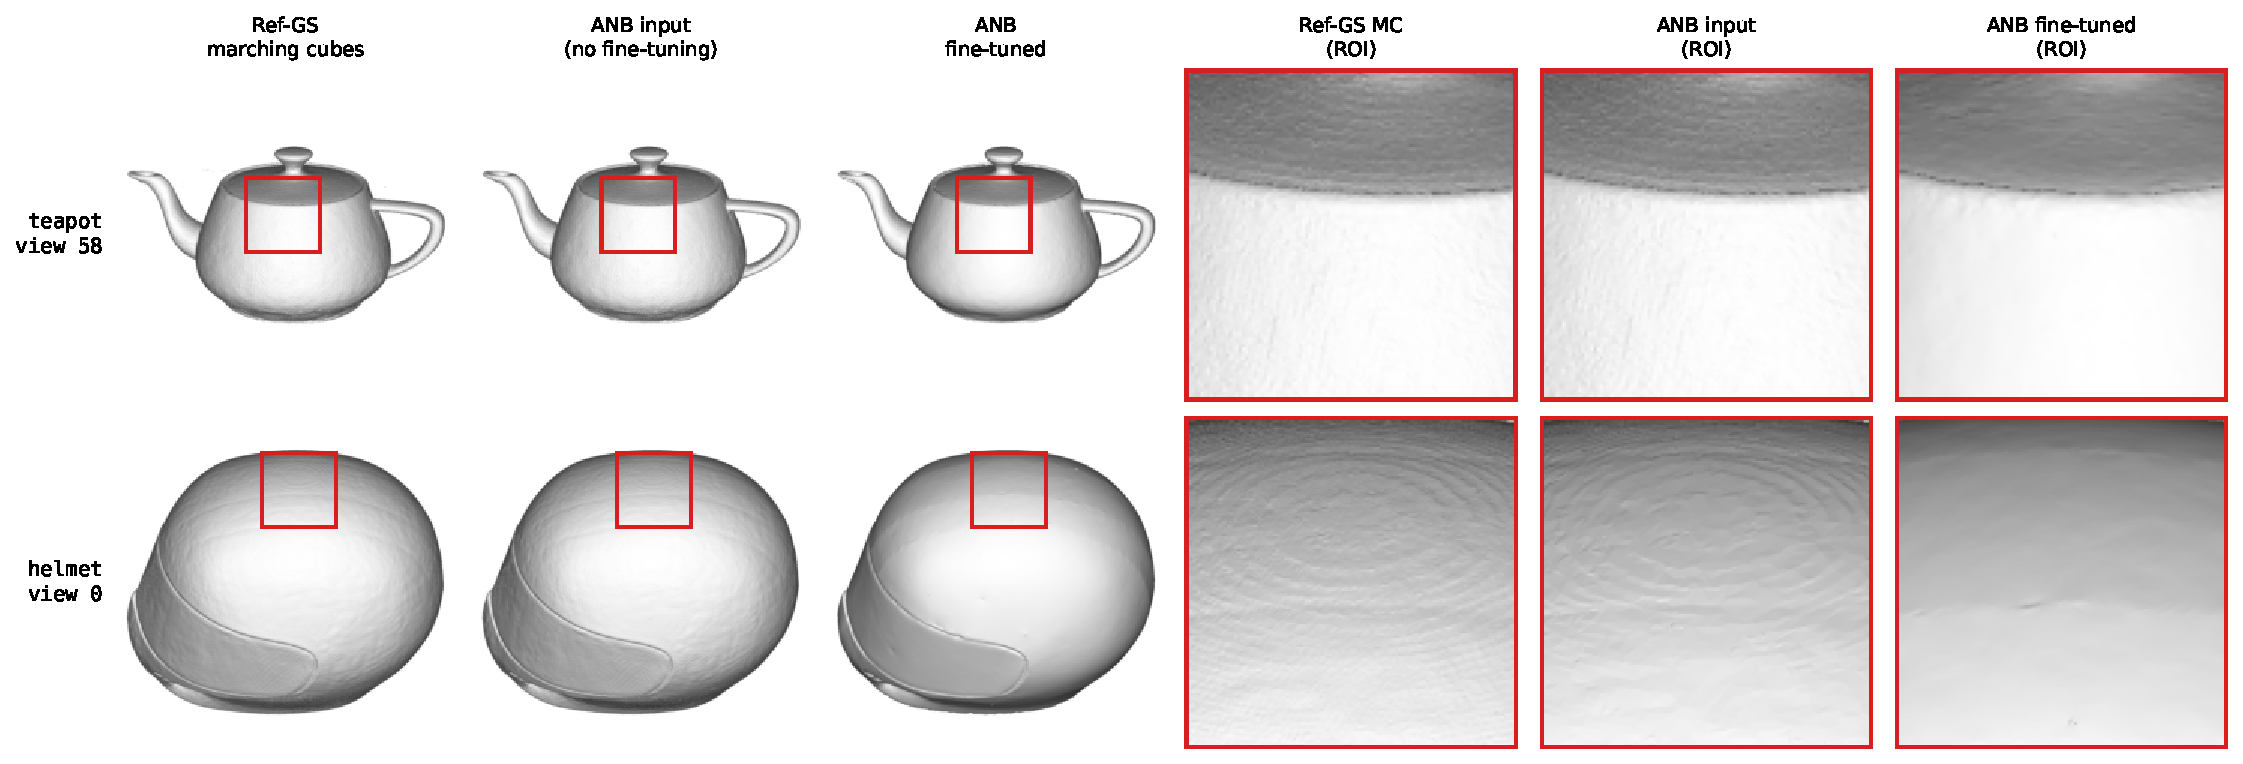
\includegraphics[width=\linewidth]{figs/mesh_ringing.pdf}
    \caption{\textbf{Effect of refinement on high-frequency surface artifacts.} Rows: \emph{teapot}
    and \emph{helmet}. Left two columns: the mesh before (input mesh) and after refinement, region of
    interest boxed in red; right two columns: the boxed region magnified. Refinement removes the
    fine noise on \emph{teapot} and the concentric ringing left by marching-cubes extraction on
    \emph{helmet}.}
    \label{fig:mesh_ringing}
\end{figure}

\begin{figure}
    \centering
    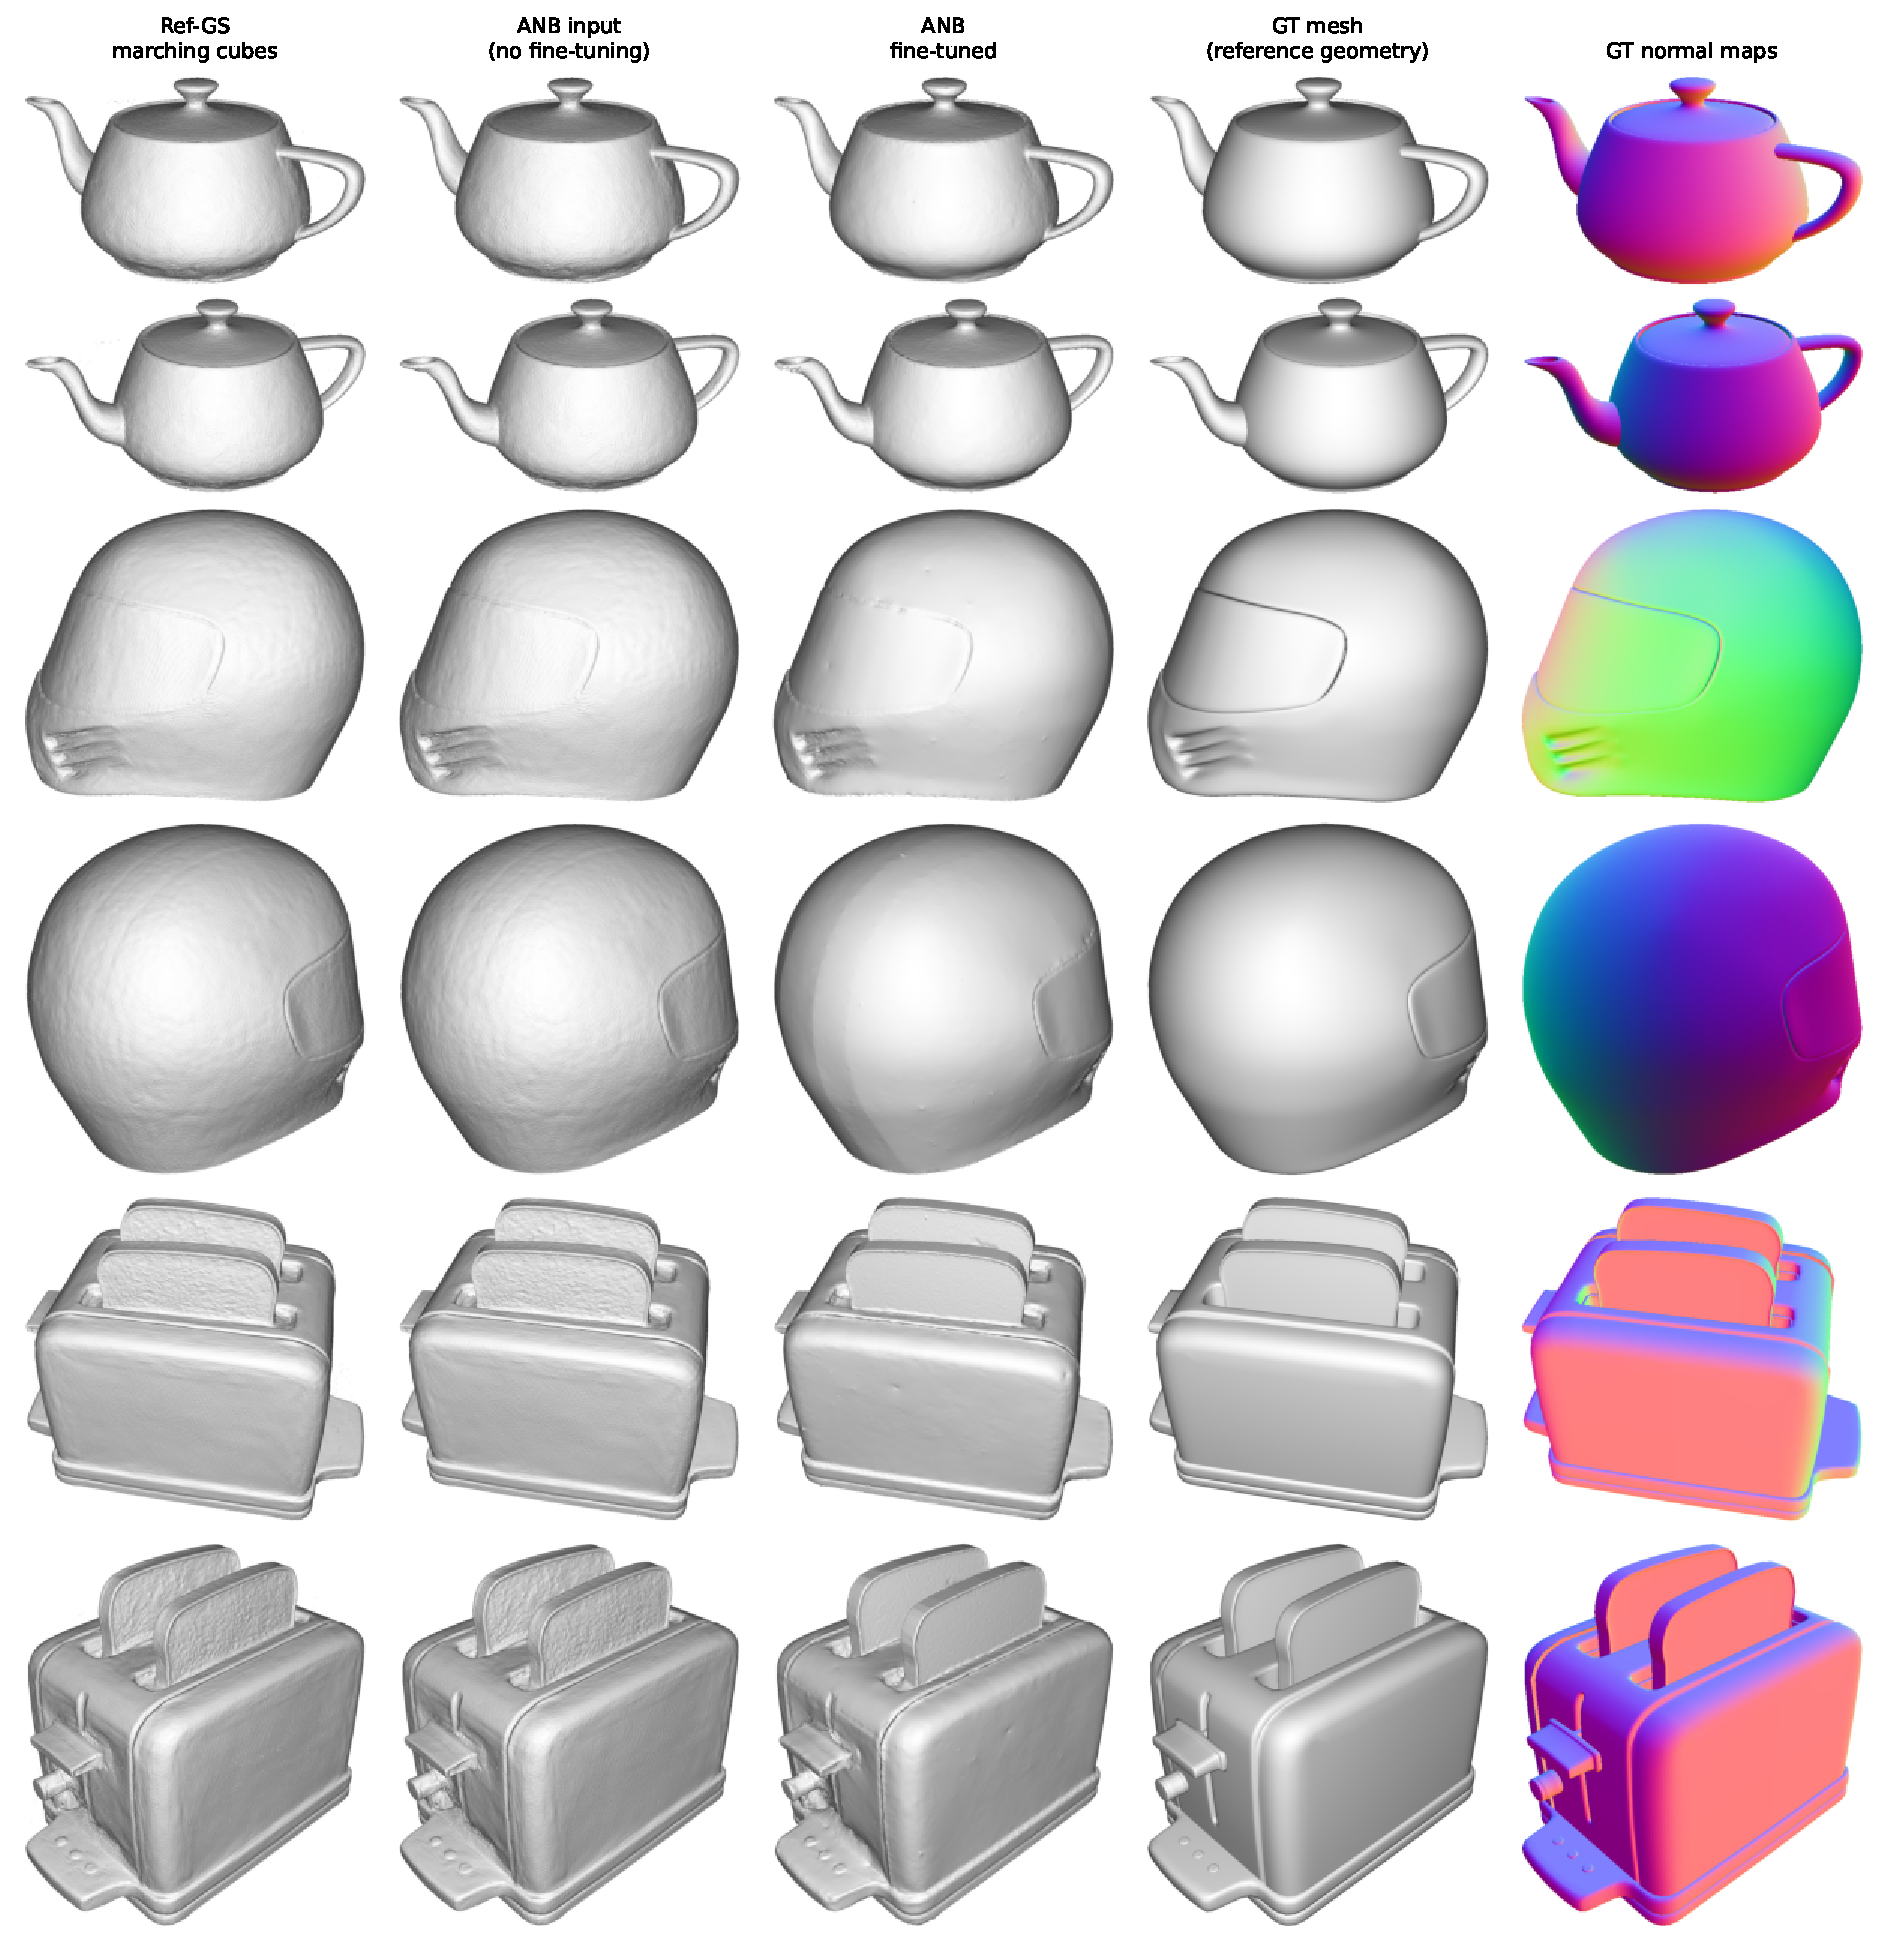
\includegraphics[width=\linewidth]{figs/mesh_qual.pdf}
    \caption{\textbf{Mesh refinement results.} Each row is one held-out test view, two each of \emph{teapot}, \emph{helmet} and \emph{toaster}. \emph{Columns 1--3} follow one mesh through our pipeline and are flat-shaded so that surface defects stay visible: (1) the mesh Ref-GS extracts by TSDF fusion and marching cubes; (2) that mesh after simplification and hole filling, which is the input to refinement; (3) the same mesh after refinement. Columns 1 and 2 differ only by simplification, so the change from column 2 to column 3 is due to refinement alone. \emph{Columns 4--5} are for reference only: the ground-truth mesh (smooth-shaded) and the ground-truth normal map for the same view.}
    \label{fig:mesh_qual}
\end{figure}

\subsection{Element-wise Compaction}
\label{app:compaction}
Because each disk is anchored independently in barycentric coordinates and carries its own albedo
and reflectivity (Sec.~\ref{sec:gmm}), it is an ordinary Gaussian splat rather than a representation-specific
primitive. This lets us apply NanoGS~\citep{nanogs}, a training-free splat simplifier developed for
free-floating 3D Gaussian Splatting, directly to our on-manifold disks with no modification: we run
it once on the trained asset to merge and prune disks down to a target fraction, with no further
optimization. Table~\ref{tab:compaction_perscene} details the per-scene results summarized in
Table~\ref{tab:compaction}. Degradation is graceful and uneven across scenes: \emph{teapot} and
\emph{ball} are essentially unaffected down to $10\%$ of the disks, while \emph{helmet}, the most
geometrically detailed scene, loses the most on every metric. This is the behavior we would expect
from an asset built out of individually addressable, mergeable elements, and it is the property a
baking pipeline needs for automatic level-of-detail generation, the splat analogue of a mipmap
chain, without a bespoke LOD method.

\begin{table}[t]
\centering
\footnotesize
\setlength{\tabcolsep}{3pt}
\caption{\textbf{Per-scene compaction results} on Shiny-Blender, same setting as
Table~\ref{tab:compaction}. Kept is the fraction of disks retained by NanoGS~\citep{nanogs}.
Avg.\ averages the per-scene values. Best value per column in \textbf{bold}.}
\label{tab:compaction_perscene}
\begin{tabular}{@{}lccccccc@{}}
\toprule
Kept & Helmet & Teapot & Toaster & Coffee & Car & Ball & Avg. \\
\midrule
\multicolumn{8}{c}{PSNR$\uparrow$} \\
\midrule
100\% & \textbf{37.94} & \textbf{47.45} & \textbf{28.76} & \textbf{35.33} & \textbf{33.75} & \textbf{45.01} & \textbf{38.04} \\
50\%  & 37.31 & \textbf{47.45} & 28.39 & 34.83 & 33.13 & 44.93 & 37.67 \\
25\%  & 36.25 & 47.26 & 27.86 & 34.11 & 32.23 & 44.94 & 37.11 \\
10\%  & 34.33 & 46.59 & 27.07 & 32.20 & 31.07 & 44.94 & 36.03 \\
\midrule
\multicolumn{8}{c}{SSIM$\uparrow$} \\
\midrule
100\% & \textbf{0.9902} & \textbf{0.9983} & \textbf{0.9607} & \textbf{0.9777} & \textbf{0.9763} & \textbf{0.9945} & \textbf{0.9830} \\
50\%  & 0.9891 & \textbf{0.9983} & 0.9500 & 0.9743 & 0.9733 & 0.9942 & 0.9799 \\
25\%  & 0.9870 & 0.9982 & 0.9388 & 0.9709 & 0.9694 & 0.9944 & 0.9764 \\
10\%  & 0.9758 & 0.9981 & 0.9262 & 0.9617 & 0.9635 & \textbf{0.9945} & 0.9700 \\
\midrule
\multicolumn{8}{c}{LPIPS$\downarrow$} \\
\midrule
100\% & \textbf{0.0130} & 0.0039 & \textbf{0.0455} & \textbf{0.0427} & \textbf{0.0154} & \textbf{0.0224} & \textbf{0.0238} \\
50\%  & 0.0172 & \textbf{0.0037} & 0.0557 & 0.0465 & 0.0186 & 0.0232 & 0.0275 \\
25\%  & 0.0220 & 0.0038 & 0.0660 & 0.0545 & 0.0231 & 0.0250 & 0.0324 \\
10\%  & 0.0565 & 0.0039 & 0.0781 & 0.0722 & 0.0289 & 0.0261 & 0.0443 \\
\bottomrule
\end{tabular}
\end{table}



\end{document}
